\pdfminorversion=4
\documentclass[aspectratio=169]{beamer}

\mode<presentation>
{
  \usetheme{default}
  \usecolortheme{default}
  \usefonttheme{default}
  \setbeamertemplate{navigation symbols}{}
  \setbeamertemplate{caption}[numbered]
  \setbeamertemplate{footline}[frame number]  % or "page number"
  \setbeamercolor{frametitle}{fg=white}
  \setbeamercolor{footline}{fg=black}
}

\usepackage[english]{babel}
\usepackage{inputenc}
\usepackage{tikz}
\usepackage{courier}
\usepackage{array}
\usepackage{bold-extra}
\usepackage{minted}
\usepackage[thicklines]{cancel}
\usepackage{fancyvrb}
\usepackage[normalem]{ulem}

\xdefinecolor{dianablue}{rgb}{0.18,0.24,0.31}
\xdefinecolor{darkblue}{rgb}{0.1,0.1,0.7}
\xdefinecolor{darkgreen}{rgb}{0,0.5,0}
\xdefinecolor{darkgrey}{rgb}{0.35,0.35,0.35}
\xdefinecolor{darkorange}{rgb}{0.8,0.5,0}
\xdefinecolor{darkred}{rgb}{0.7,0,0}
\definecolor{darkgreen}{rgb}{0,0.6,0}
\definecolor{mauve}{rgb}{0.58,0,0.82}

\title[2024-07-24-codas-hep-ml-01]{Machine learning at CoDaS-HEP 2024}
\author{Jim Pivarski}
\institute{Princeton University -- IRIS-HEP}
\date{July 25, 2024}

\usetikzlibrary{shapes.callouts}

\begin{document}

\logo{\pgfputat{\pgfxy(0.11, 7.4)}{\pgfbox[right,base]{\tikz{\filldraw[fill=dianablue, draw=none] (0 cm, 0 cm) rectangle (50 cm, 1 cm);}\mbox{\hspace{-8 cm}
\includegraphics[height=1 cm]{princeton-logo-long.png}\hspace{0.1 cm}\raisebox{0.1 cm}{
\includegraphics[height=0.8 cm]{iris-hep-logo-long.png}}\hspace{0.1 cm}}}}}

\begin{frame}
  \titlepage
\end{frame}

\logo{\pgfputat{\pgfxy(0.11, 7.4)}{\pgfbox[right,base]{\tikz{\filldraw[fill=dianablue, draw=none] (0 cm, 0 cm) rectangle (50 cm, 1 cm);}\mbox{\hspace{-8 cm}
\includegraphics[height=1 cm]{princeton-logo.png}\hspace{0.1 cm}\raisebox{0.1 cm}{
\includegraphics[height=0.8 cm]{iris-hep-logo.png}}\hspace{0.1 cm}}}}}

% Uncomment these lines for an automatically generated outline.
%\begin{frame}{Outline}
%  \tableofcontents
%\end{frame}

% START START START START START START START START START START START START START

\begin{frame}{Now we have two ways to make computer programs}
\vspace{-0.5 cm}

\begin{columns}[t]
\column{0.5\linewidth}
\begin{center}
\Large Craftsmanship

\vspace{0.25 cm}
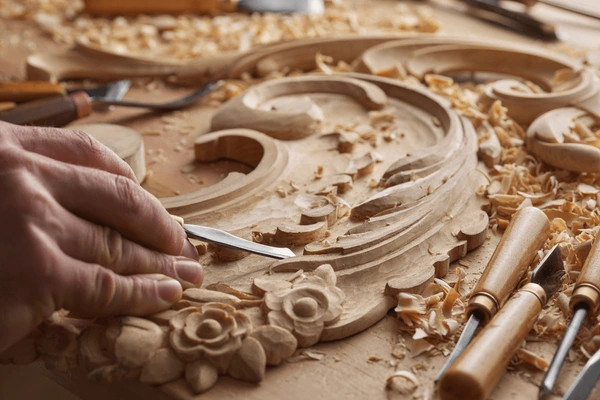
\includegraphics[width=0.8\linewidth]{img/craftsmanship.jpg}

\normalsize
\vspace{0.25 cm}
\begin{itemize}
\item Programming ``by hand''
\item Allows for precise control
\item Complexity limited by a human mind or a team's ability to communicate
\end{itemize}
\end{center}

\column{0.5\linewidth}
\begin{center}
\Large Farming

\vspace{0.25 cm}
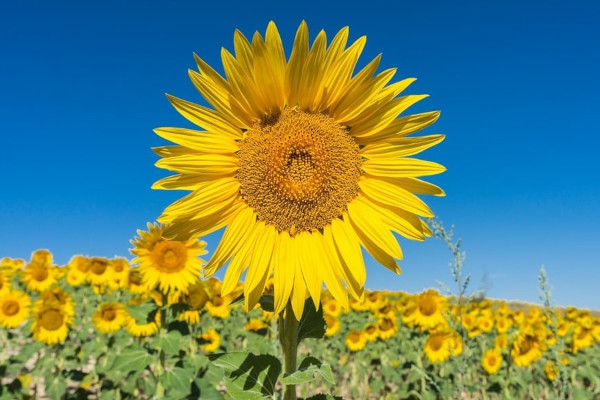
\includegraphics[width=0.8\linewidth]{img/farming.jpg}

\normalsize
\vspace{0.25 cm}
\begin{itemize}
\item Machine learning
\item Allows for extremely nuanced solutions
\item Still needs human help to steer it toward the ``right'' solution
\end{itemize}
\end{center}

\end{columns}
\end{frame}

\begin{frame}{Machine learning in a nutshell}
\vspace{0.4 cm}
\Large

Write an algorithm that generates output that depends on a huge number of internal parameters.

\vspace{0.5 cm}
\uncover<2->{Vary those parameters until the algorithm returns the expected result (supervised learning) or until it finds patterns according to some desired metric (unsupervised learning).}

\vspace{0.5 cm}
\uncover<3->{Then use the trained algorithm on new problems.}

\vspace{0.5 cm}
\uncover<4->{\textcolor{darkblue}{If this sounds like fitting data with a function, you're right.}}
\end{frame}

\begin{frame}{Goals of this mini-course}
\vspace{0.4 cm}
\Large

\begin{enumerate}\setlength{\itemsep}{0.5 cm}
\item Understand how your physics background prepares you for machine learning.
\item Don't approach it as a black box/dark art.
\item Get a little familiar with some common tools and techniques.
\end{enumerate}
\end{frame}

\begin{frame}{A very brief history of HEP and ML}
\Large
\vspace{0.5 cm}
\begin{columns}
\column{0.5\linewidth}
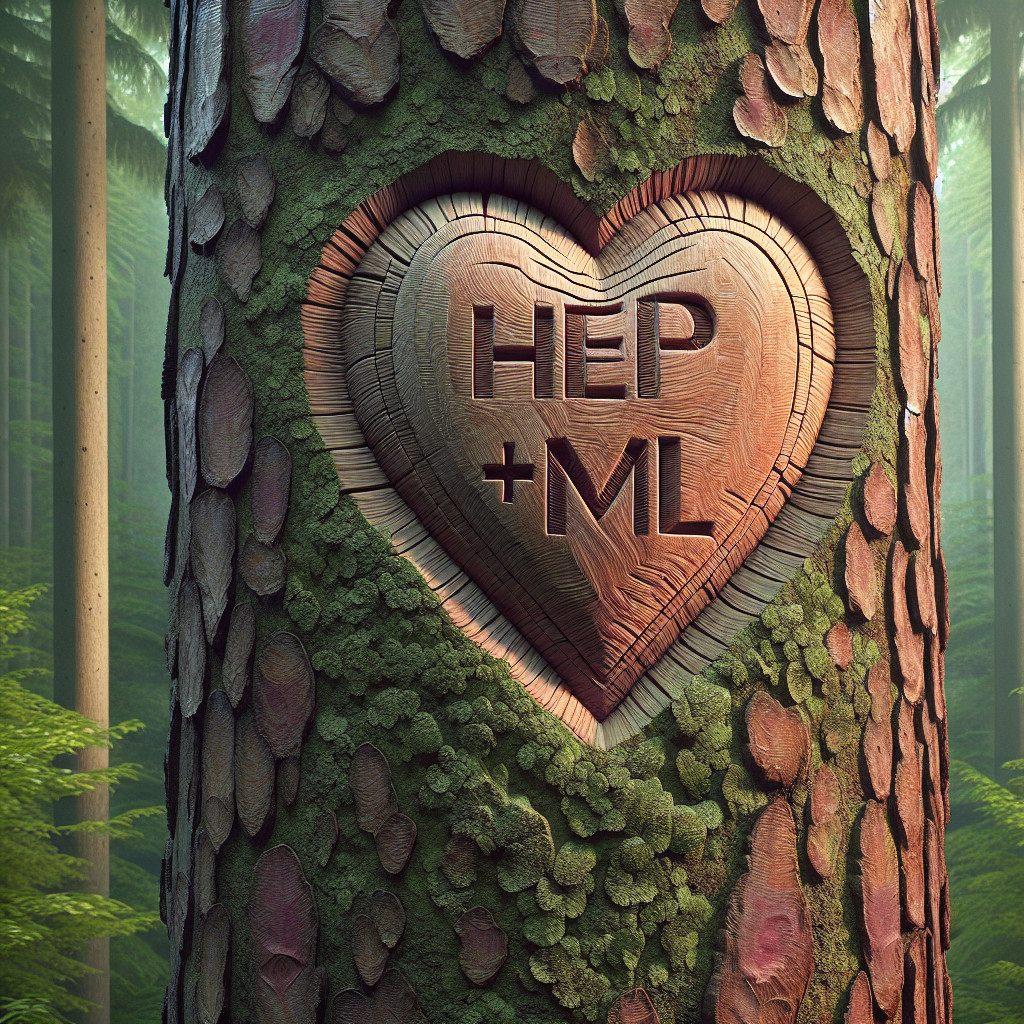
\includegraphics[width=\linewidth]{img/hep-plus-ml.jpg}

\column{0.5\linewidth}
Main point: High Energy Physics (HEP) has always needed Machine Learning (ML).

\vspace{0.5 cm}
It's just becoming {\it possible} now.
\end{columns}
\end{frame}

\begin{frame}{First HEP experiments adopted computers in a major way}
\vspace{0.35 cm}
\large

Late 1940's---early 1950's was the ``beginning'' of HEP as we know it:

\vspace{0.25 cm}
\begin{itemize}
\item Accelerators provided higher energy with higher flux than observed in nature.
\item Collisions with fixed targets produced new particles to discover.
\item Computers quantified particle trajectories, reconstructed invisible (neutral) particles, and rejected backgrounds.
\end{itemize}

\normalsize
\vspace{0.35 cm}
Example: Luis Alvarez's group \textcolor{darkgreen}{\$9M} accelerator, \textcolor{darkgreen}{\$2M} bubble chamber, \textcolor{darkgreen}{\$0.2M} IBM 650.

\vspace{0.25 cm}
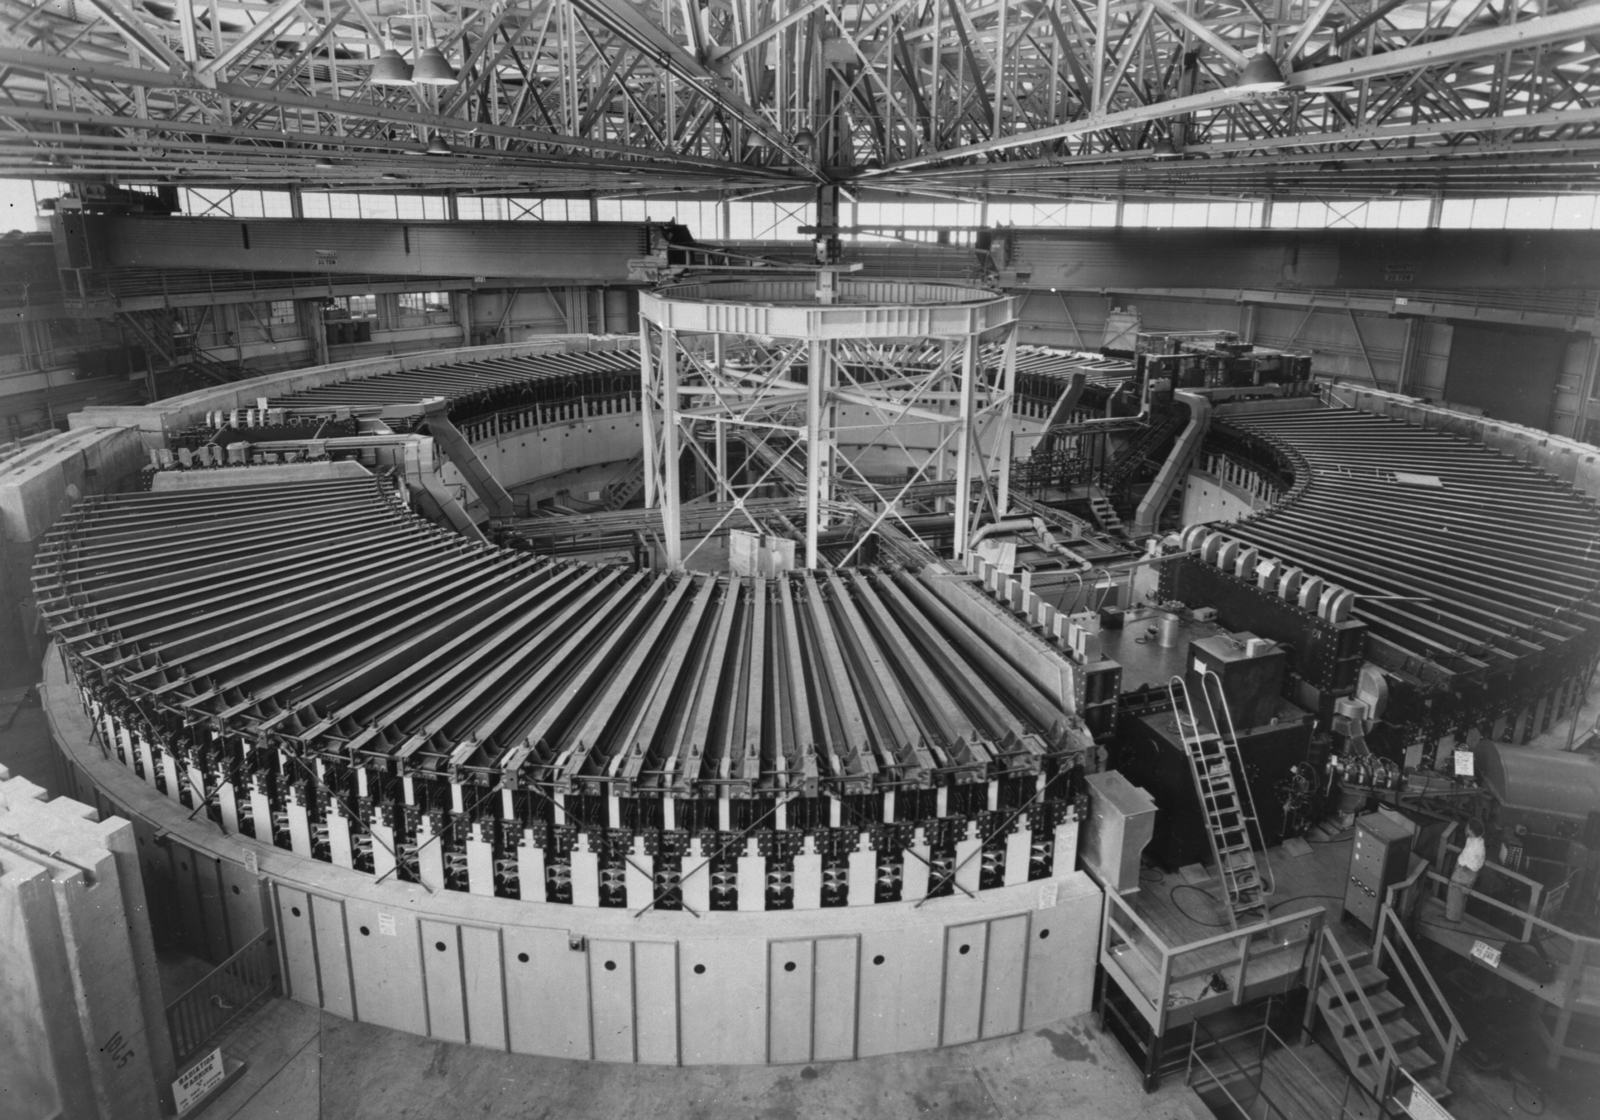
\includegraphics[height=3 cm]{img/overall-view-of-bevatron-magnet-photograph-taken-september-6-1955-bevatron-088cb0-1600.jpg}
\hfill 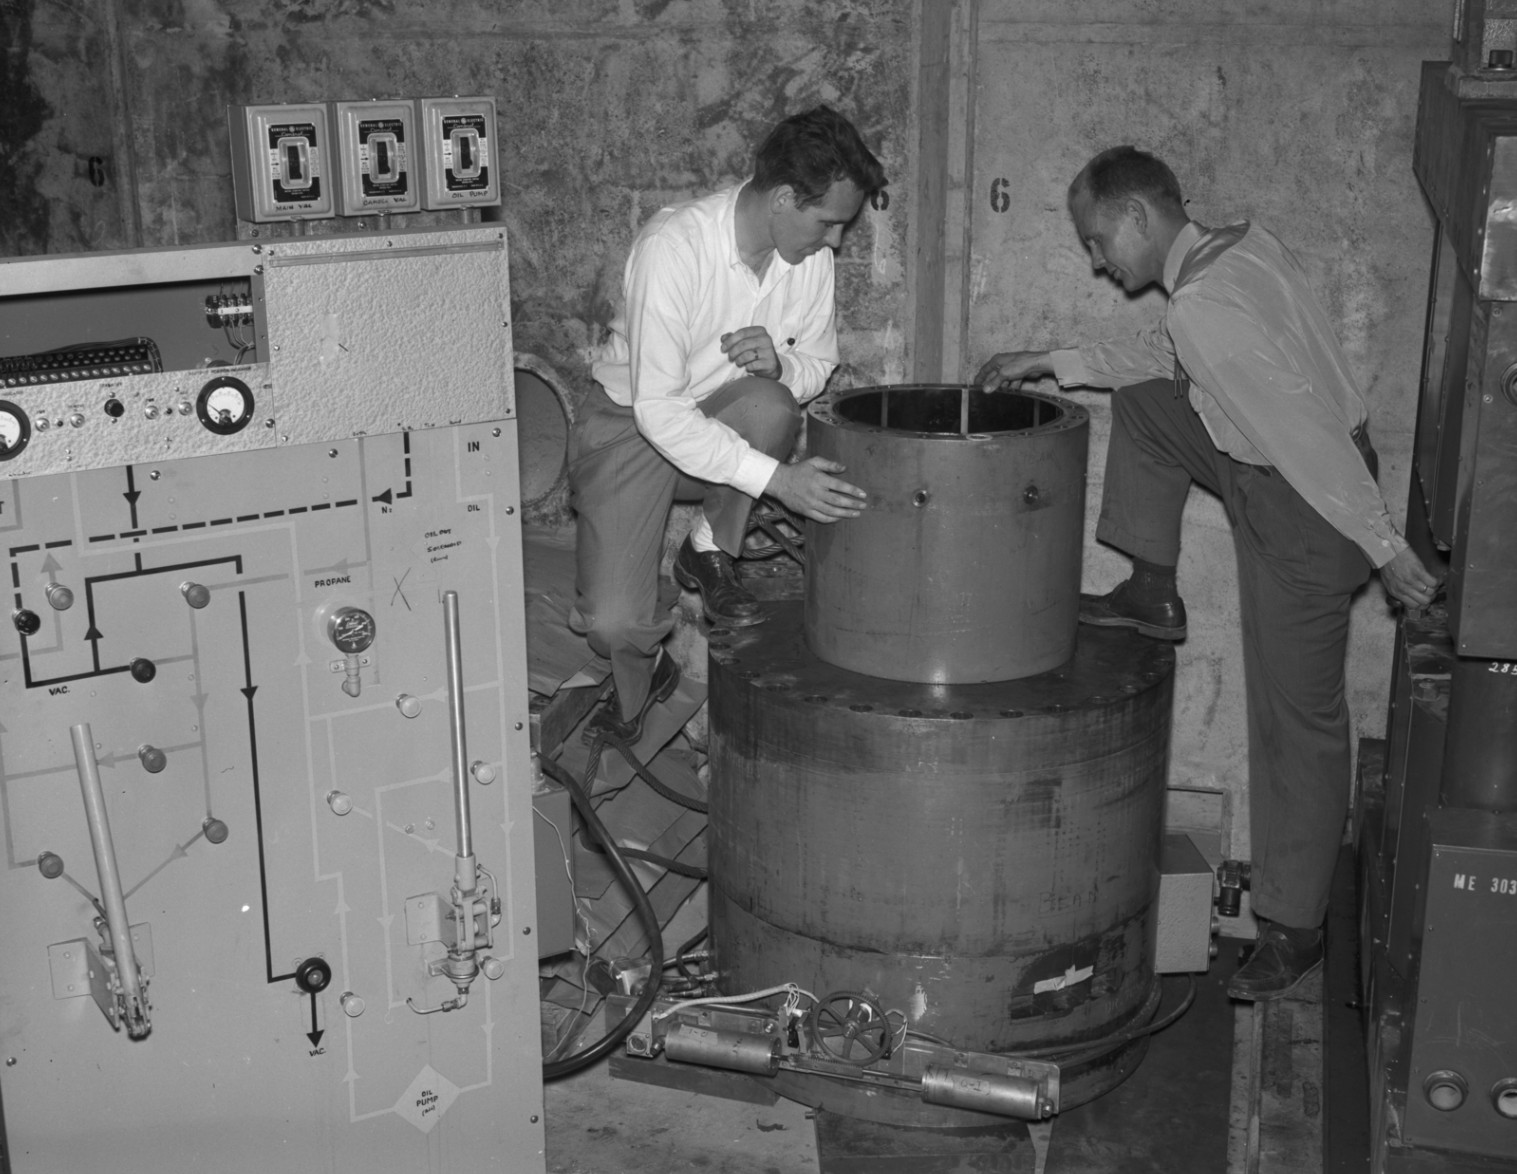
\includegraphics[height=3 cm]{img/alvarez-group-bubble-chamber.jpg}
\hfill 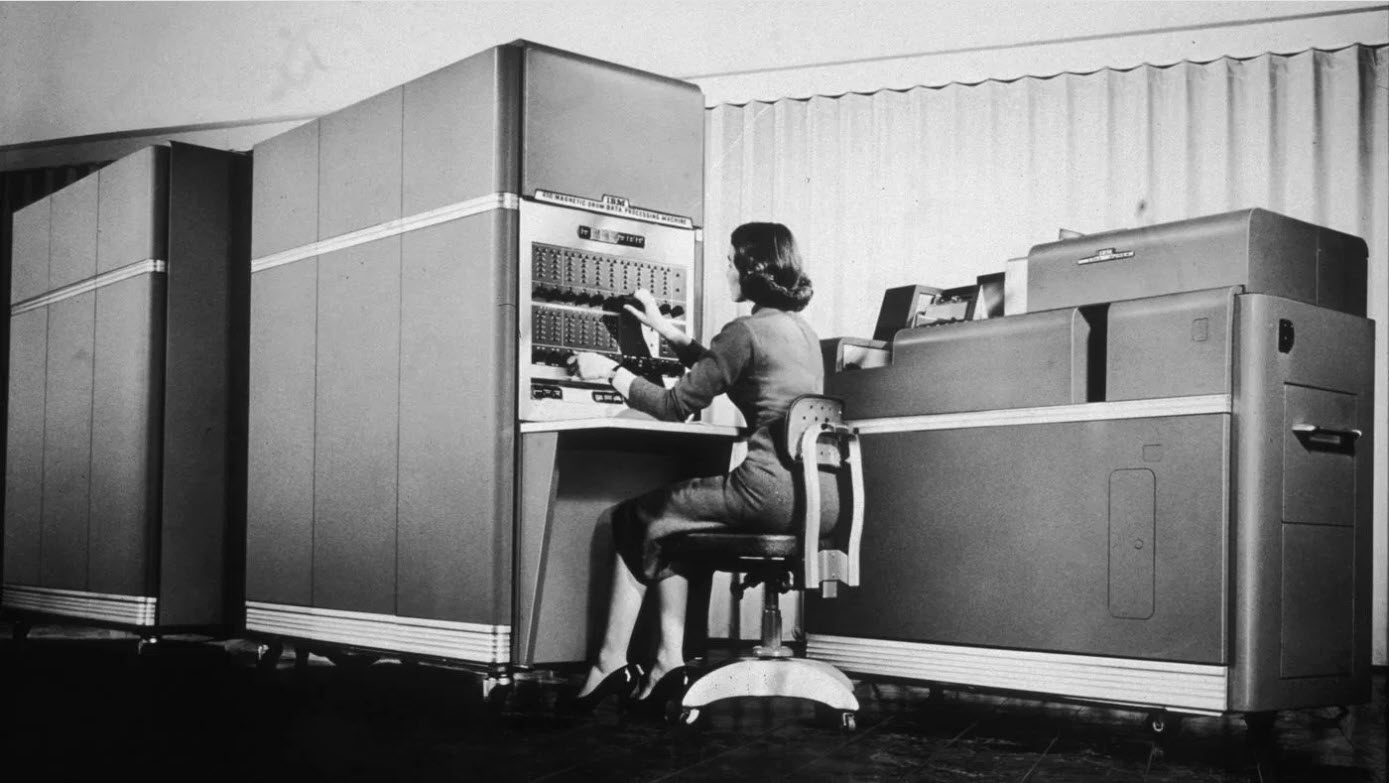
\includegraphics[height=3 cm]{img/ibm-650.jpg}
\end{frame}

\begin{frame}{Identifying tracks was beyond the capabilities of software}
\vspace{0.35 cm}
\begin{columns}
\column{0.7\linewidth}
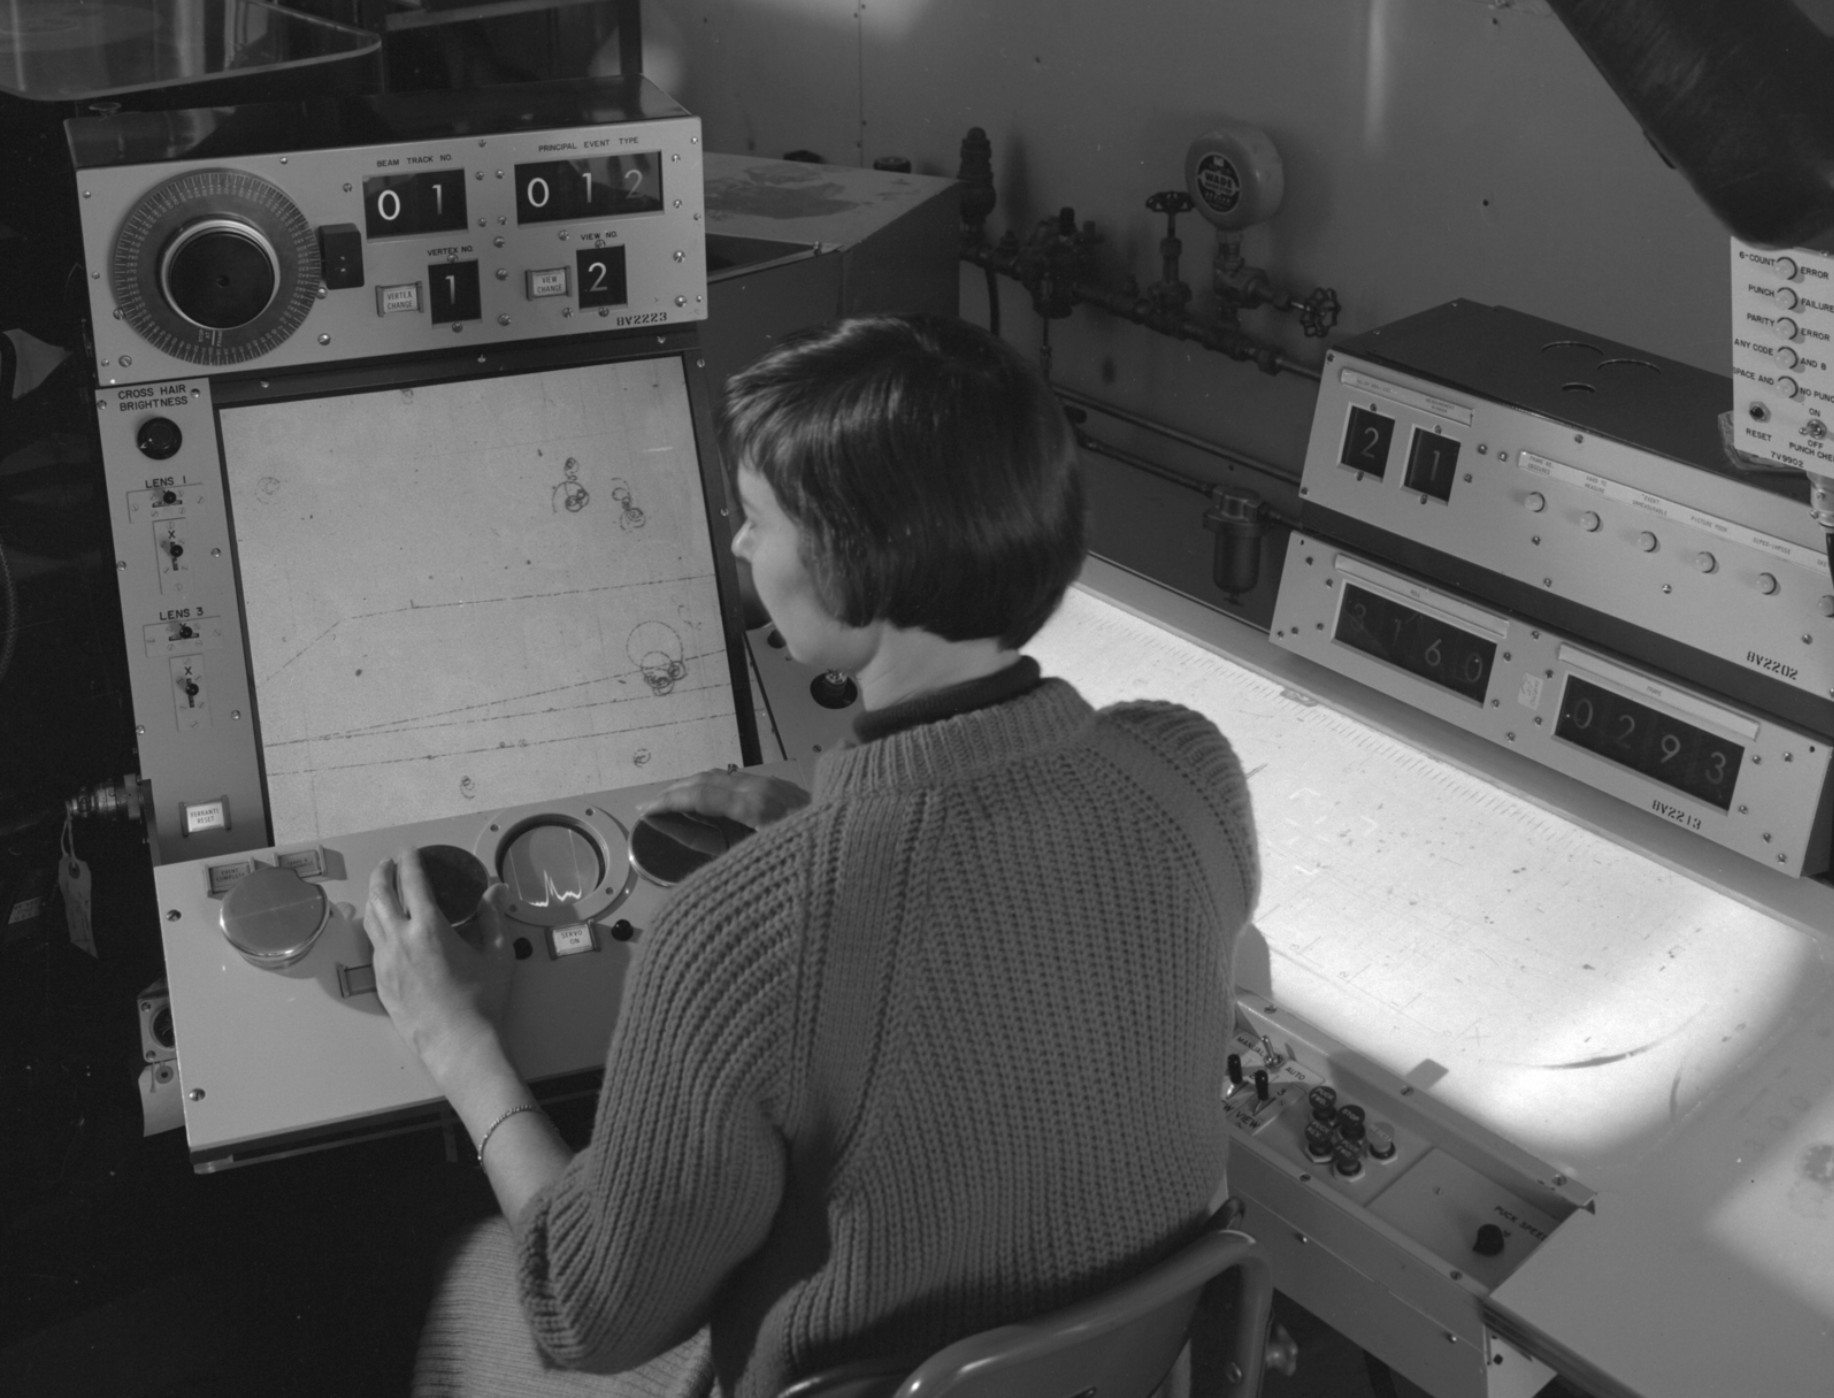
\includegraphics[width=\linewidth]{img/franckenstein-3.jpg}

\column{0.3\linewidth}
\vspace{-0.5 cm}
\begin{center}
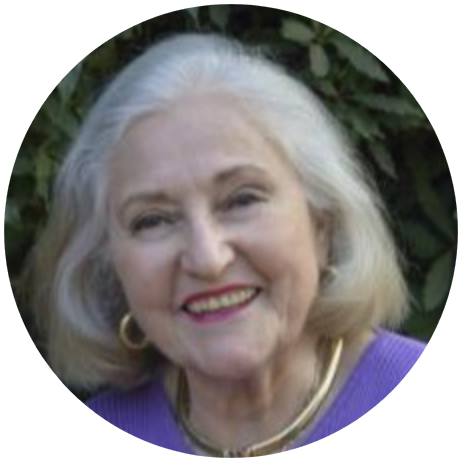
\includegraphics[width=0.5\linewidth]{img/madeleine-isenberg-SCANNER.png}

\scriptsize
Madeleine (n\'ee Goldstein) Isenberg, UCLA class of '65
\end{center}

\begin{minipage}{\linewidth}
\scriptsize
``We scanners would review each frame of film, and per the brief instructions we had been given, looked for any `unusual activity.'

\vspace{0.25 cm}
``The scanner had to use both hands, a joystick in each, and turn them clockwise or anti-clockwise, to align a double crosshair cursor at several sequential positions on a track.''

\vspace{0.25 cm}
\tiny
\textcolor{blue}{\url{https://www.physics.ucla.edu/marty/HighEnergyPhysics.pdf}}
\end{minipage}
\end{columns}
\end{frame}

\begin{frame}{Fast pattern recognition tasks are an essential part of HEP}
\vspace{0.4 cm}
\begin{columns}
\column{0.25\linewidth}
\only<1>{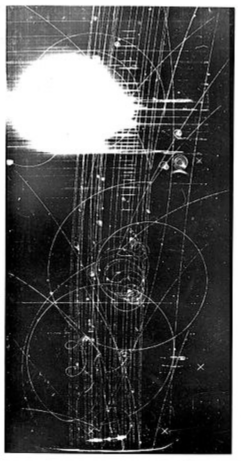
\includegraphics[height=7.5 cm]{img/bubble-chamber-photo-0.pdf}}\only<2->{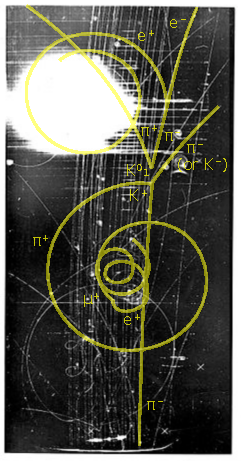
\includegraphics[height=7.5 cm]{img/bubble-chamber-photo.pdf}}

\column{0.2\linewidth}
Detectors make uninterpreted event displays.

\vspace{0.5 cm}
\uncover<2->{Raw signals must be interpreted as particles.}

\vspace{0.5 cm}
\uncover<3->{Capacity for discovery scales with the number of interpreted events.}

\column{0.4\linewidth}
\uncover<3->{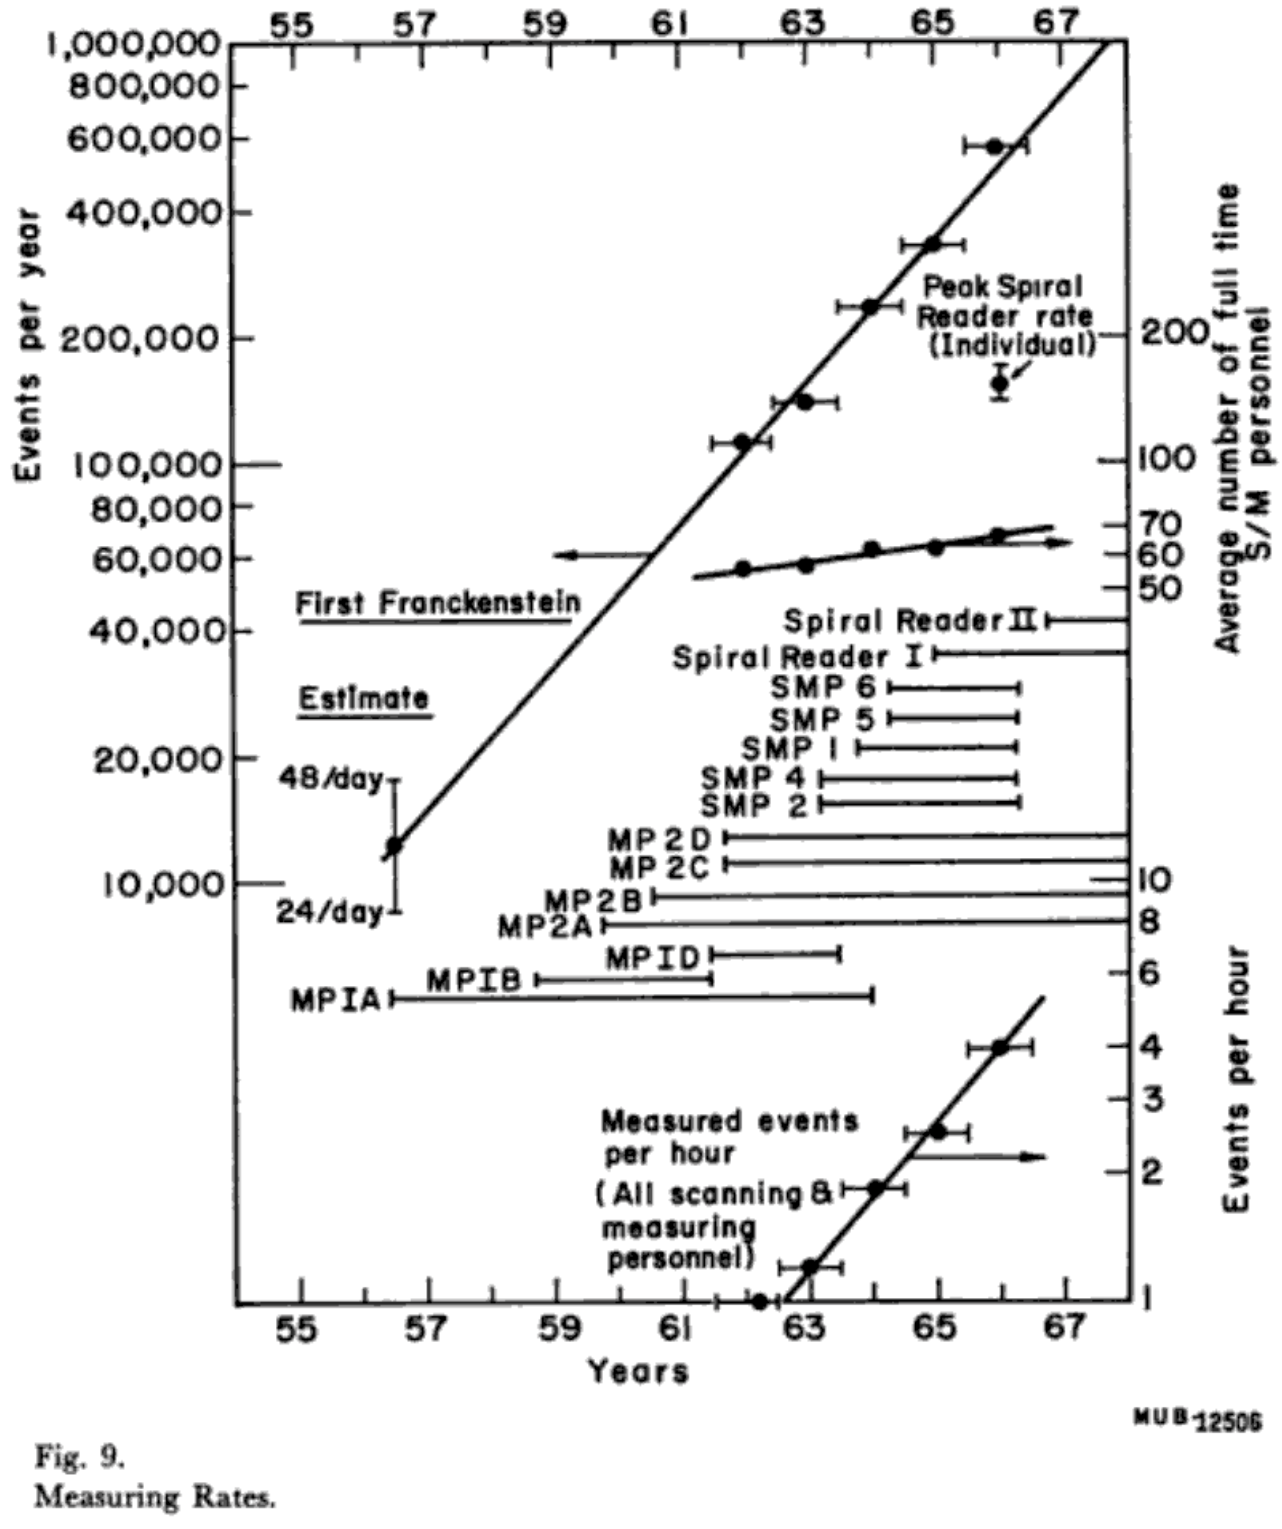
\includegraphics[height=7.5 cm]{img/scaleup.png}}
\end{columns}
\end{frame}

\begin{frame}{Pattern recognition had to be automated to reach today's rates}
\vspace{0.25 cm}
\begin{columns}
\column{1.1\linewidth}
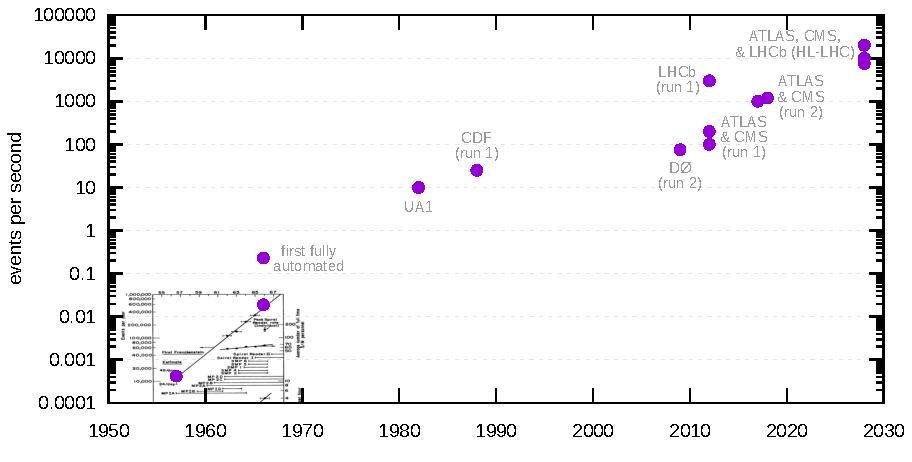
\includegraphics[width=\linewidth]{img/event-rates.pdf}
\end{columns}
\end{frame}

\begin{frame}{\mbox{ }}
\vspace{0.5 cm}
\Large

Until recently, most HEP pattern-recognition consisted of hand-written heuristics (some still is).

\vspace{1 cm}
\uncover<2->{The history of Artificial Intelligence (AI) is also split between what we would now call hand-written algorithms and learned algorithms.}
\end{frame}

\begin{frame}{Symbolic AI versus Connectionist AI}
\vspace{-0.7 cm}

\begin{columns}[t]
\column{0.5\linewidth}
\begin{center}
\Large Symbolic

\vspace{0.25 cm}
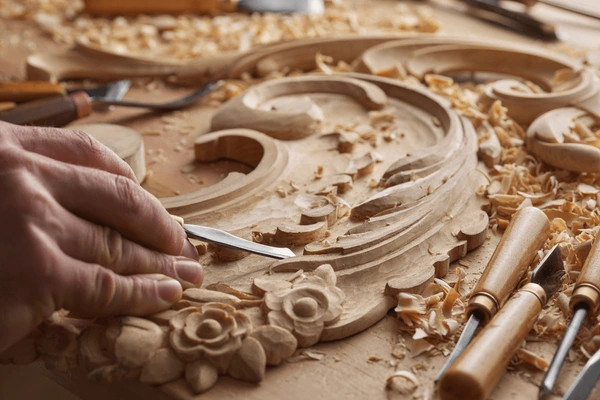
\includegraphics[width=0.8\linewidth]{img/craftsmanship.jpg}

\normalsize
\vspace{0.25 cm}
\begin{itemize}
\item Symbol manipulation and logic
\item Searches through problem-space
\item Hand-written common-sense rules
\end{itemize}

Examples: parsing, theorem-proving, chess-playing, expert systems
\end{center}

\column{0.5\linewidth}
\begin{center}
\Large Connectionist

\vspace{0.25 cm}
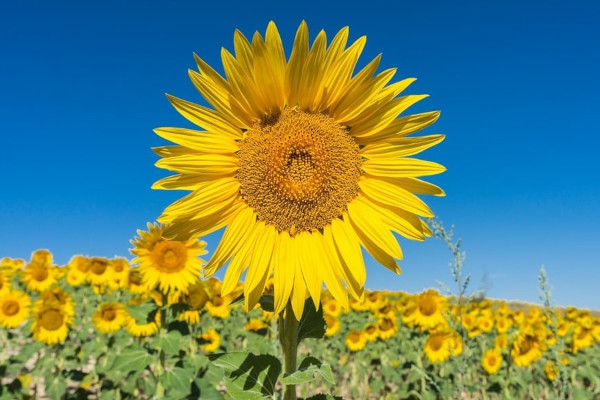
\includegraphics[width=0.8\linewidth]{img/farming.jpg}

\normalsize
\vspace{0.25 cm}
\begin{itemize}
\item Stimulus correlated to response only by strengths of internal connections
\item No \underline{\it explicit} symbols or rules
\item \underline{\it Effective} symbols/rules may arise
\end{itemize}

Examples: neural networks
\end{center}

\end{columns}
\end{frame}

\begin{frame}{Connectionism started early}
\small
\vspace{0.2 cm}
\begin{columns}
\column{0.4\linewidth}
\includegraphics[width=\linewidth]{img/330-PSA-80-60_\(USN_710739\)_\(20897323365\).jpg}

\vspace{0.2 cm}
Theory: Pitts \& McCullock (1943).

\vspace{0.2 cm}
Rosenblatt's perceptron machine (1958) attempted to recognize images of letters by adjusting free parameters with motors.

\vspace{0.2 cm}
\mbox{\textcolor{darkorange}{\bf Made extravagant claims; reality hit hard.}\hspace{-1 cm}}

\column{0.6\linewidth}
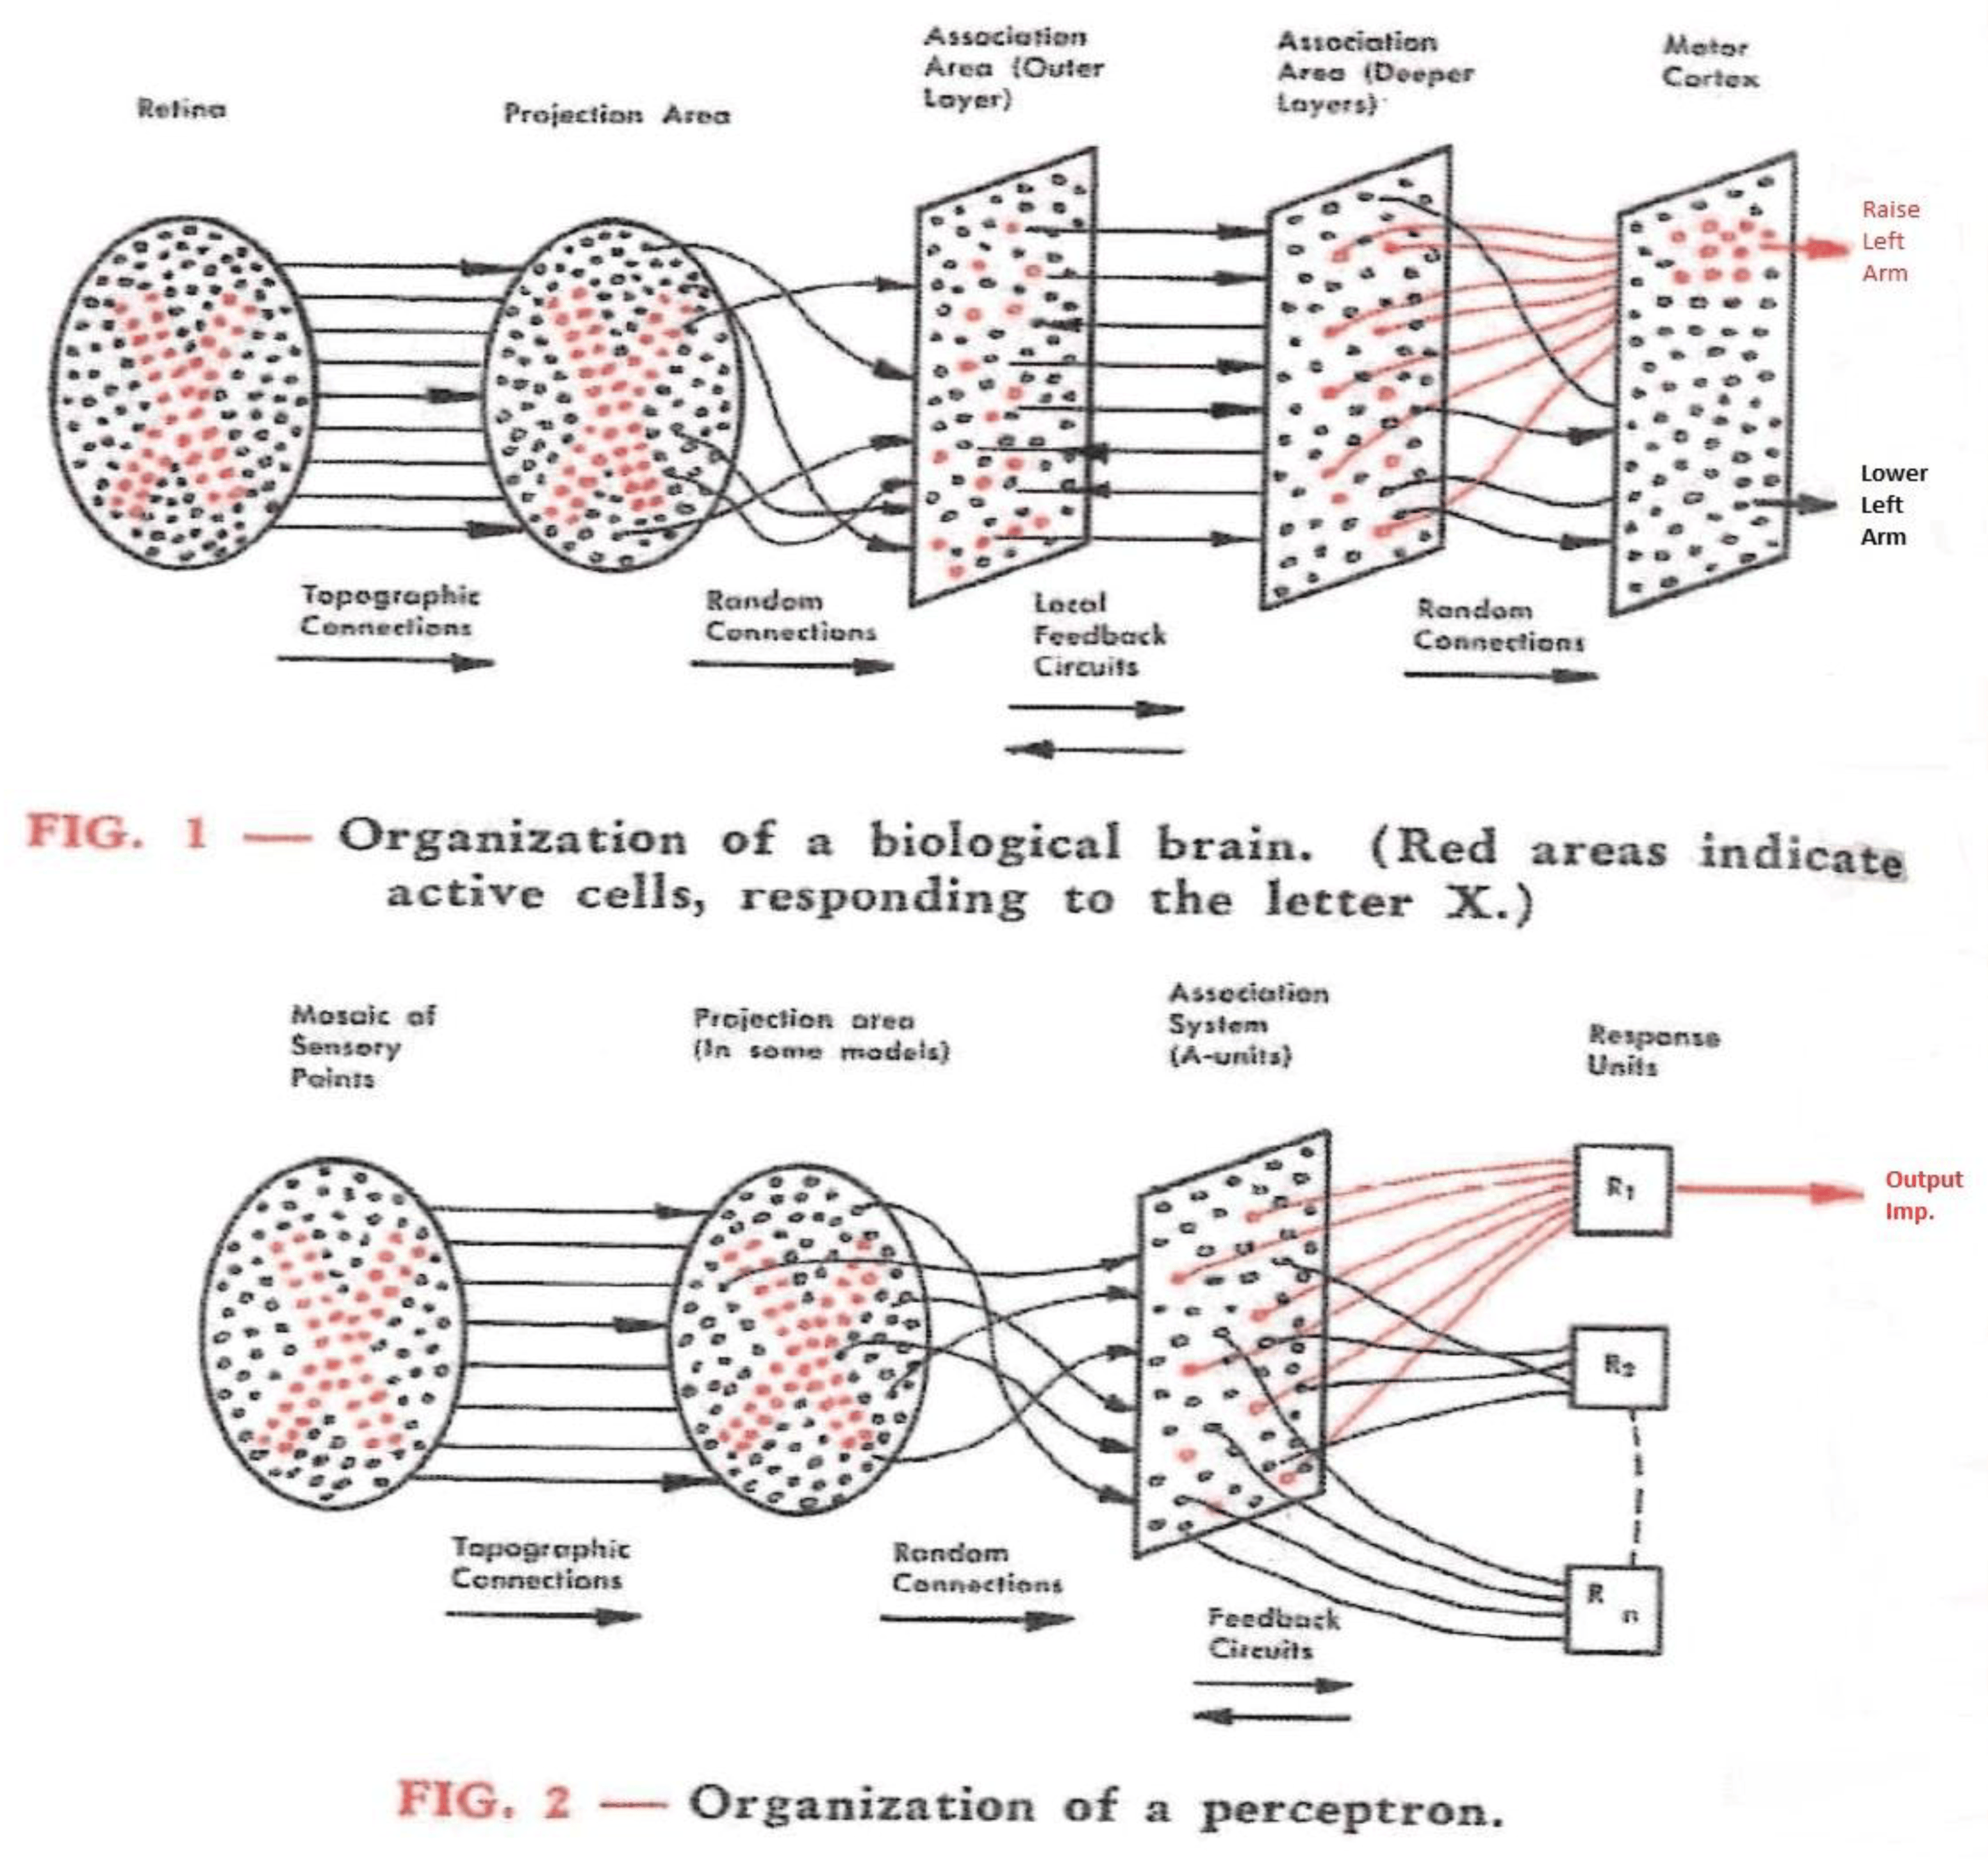
\includegraphics[width=\linewidth]{img/Organization_of_a_biological_brain_and_a_perceptron.png}
\end{columns}
\end{frame}

\begin{frame}{The ups and downs of AI: \only<1>{as mentioned in books}\only<2>{according to Henry Kautz (funding)}}
\vspace{0.2 cm}
\begin{columns}
\column{1.1\linewidth}
\only<1>{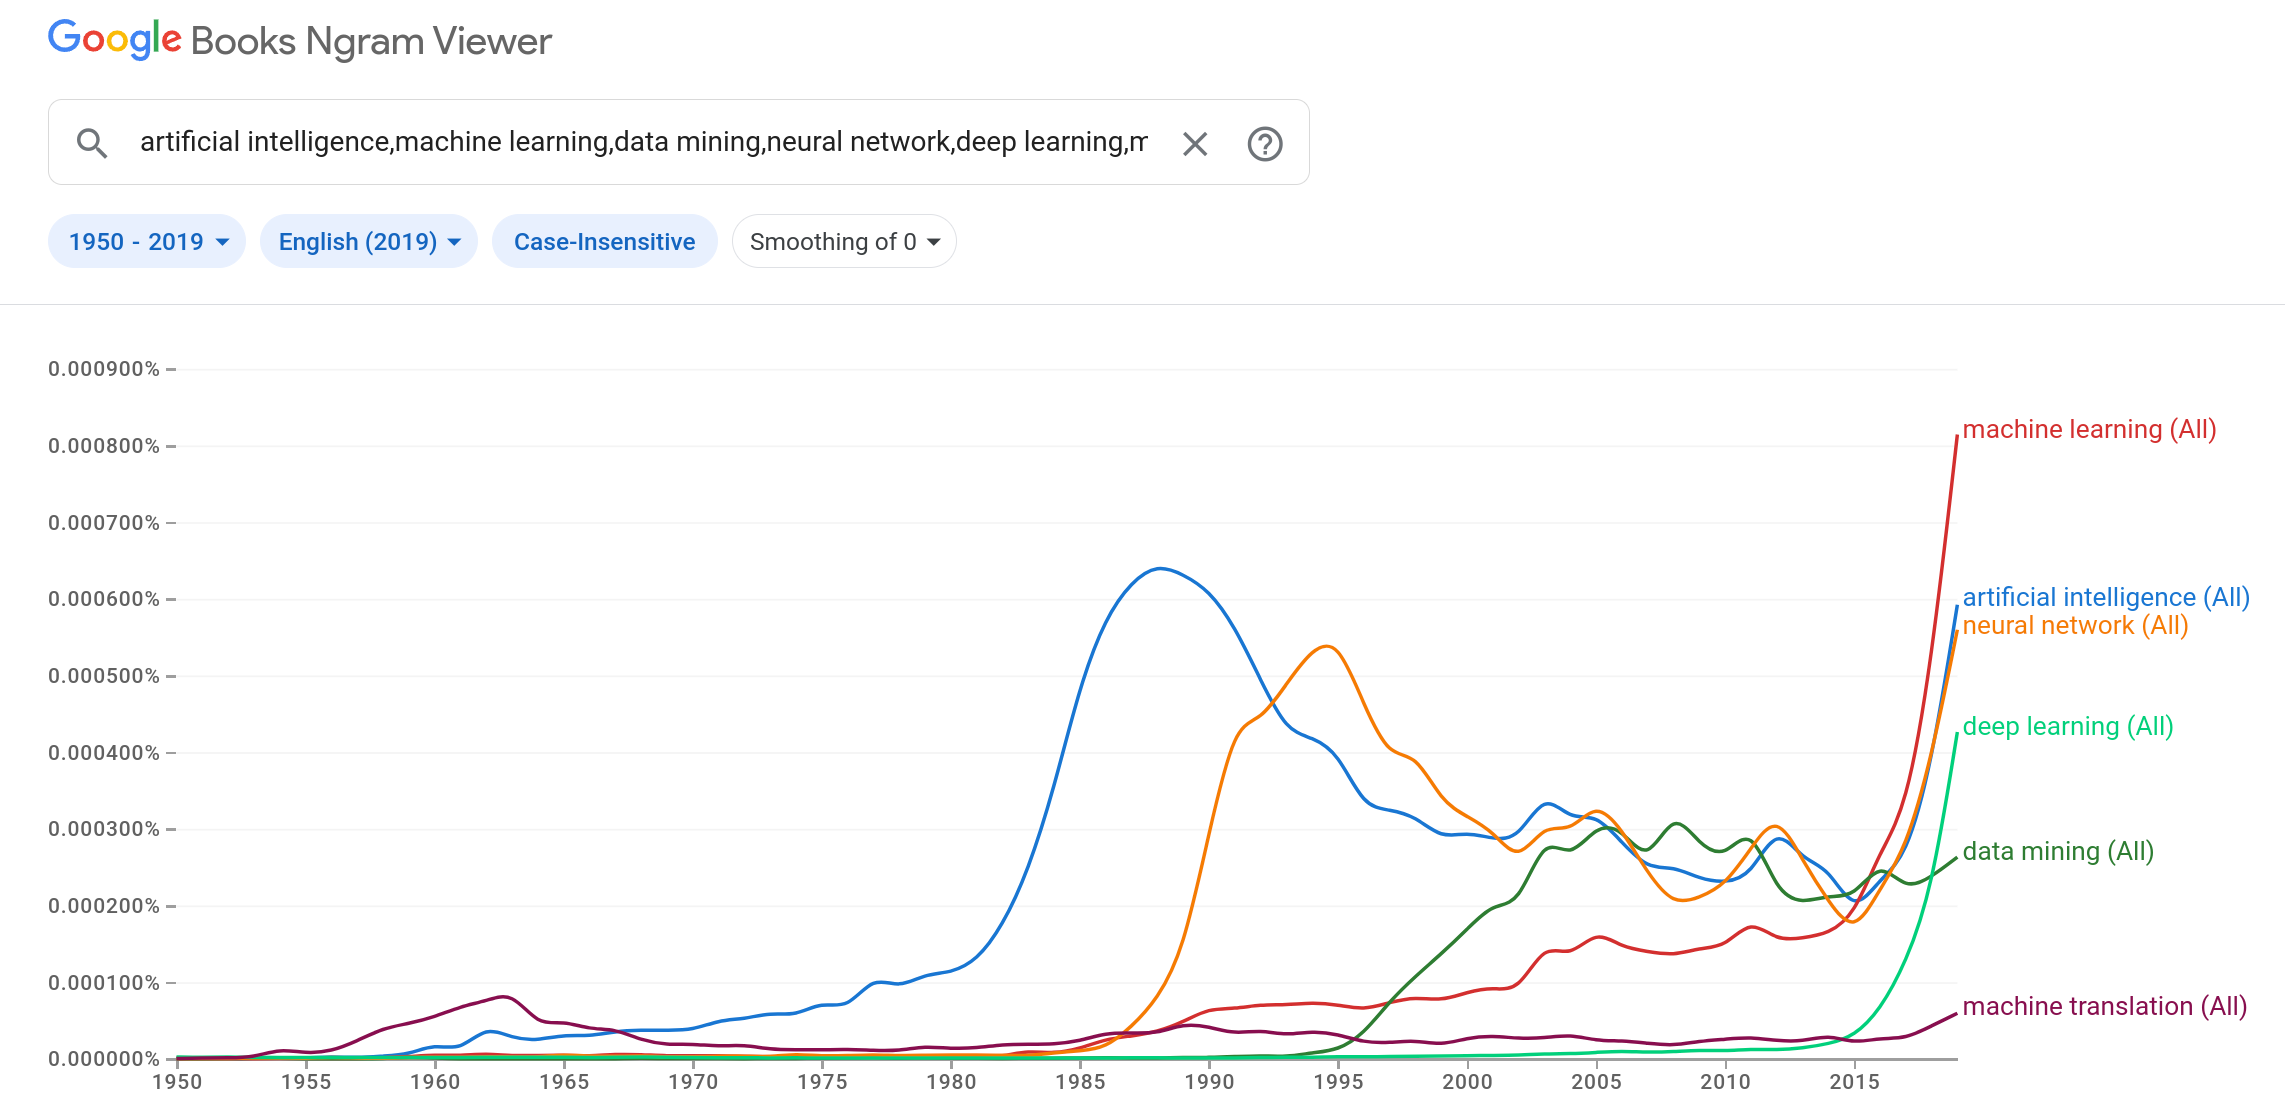
\includegraphics[width=\linewidth]{img/ups-and-downs-of-ai.png}}\only<2>{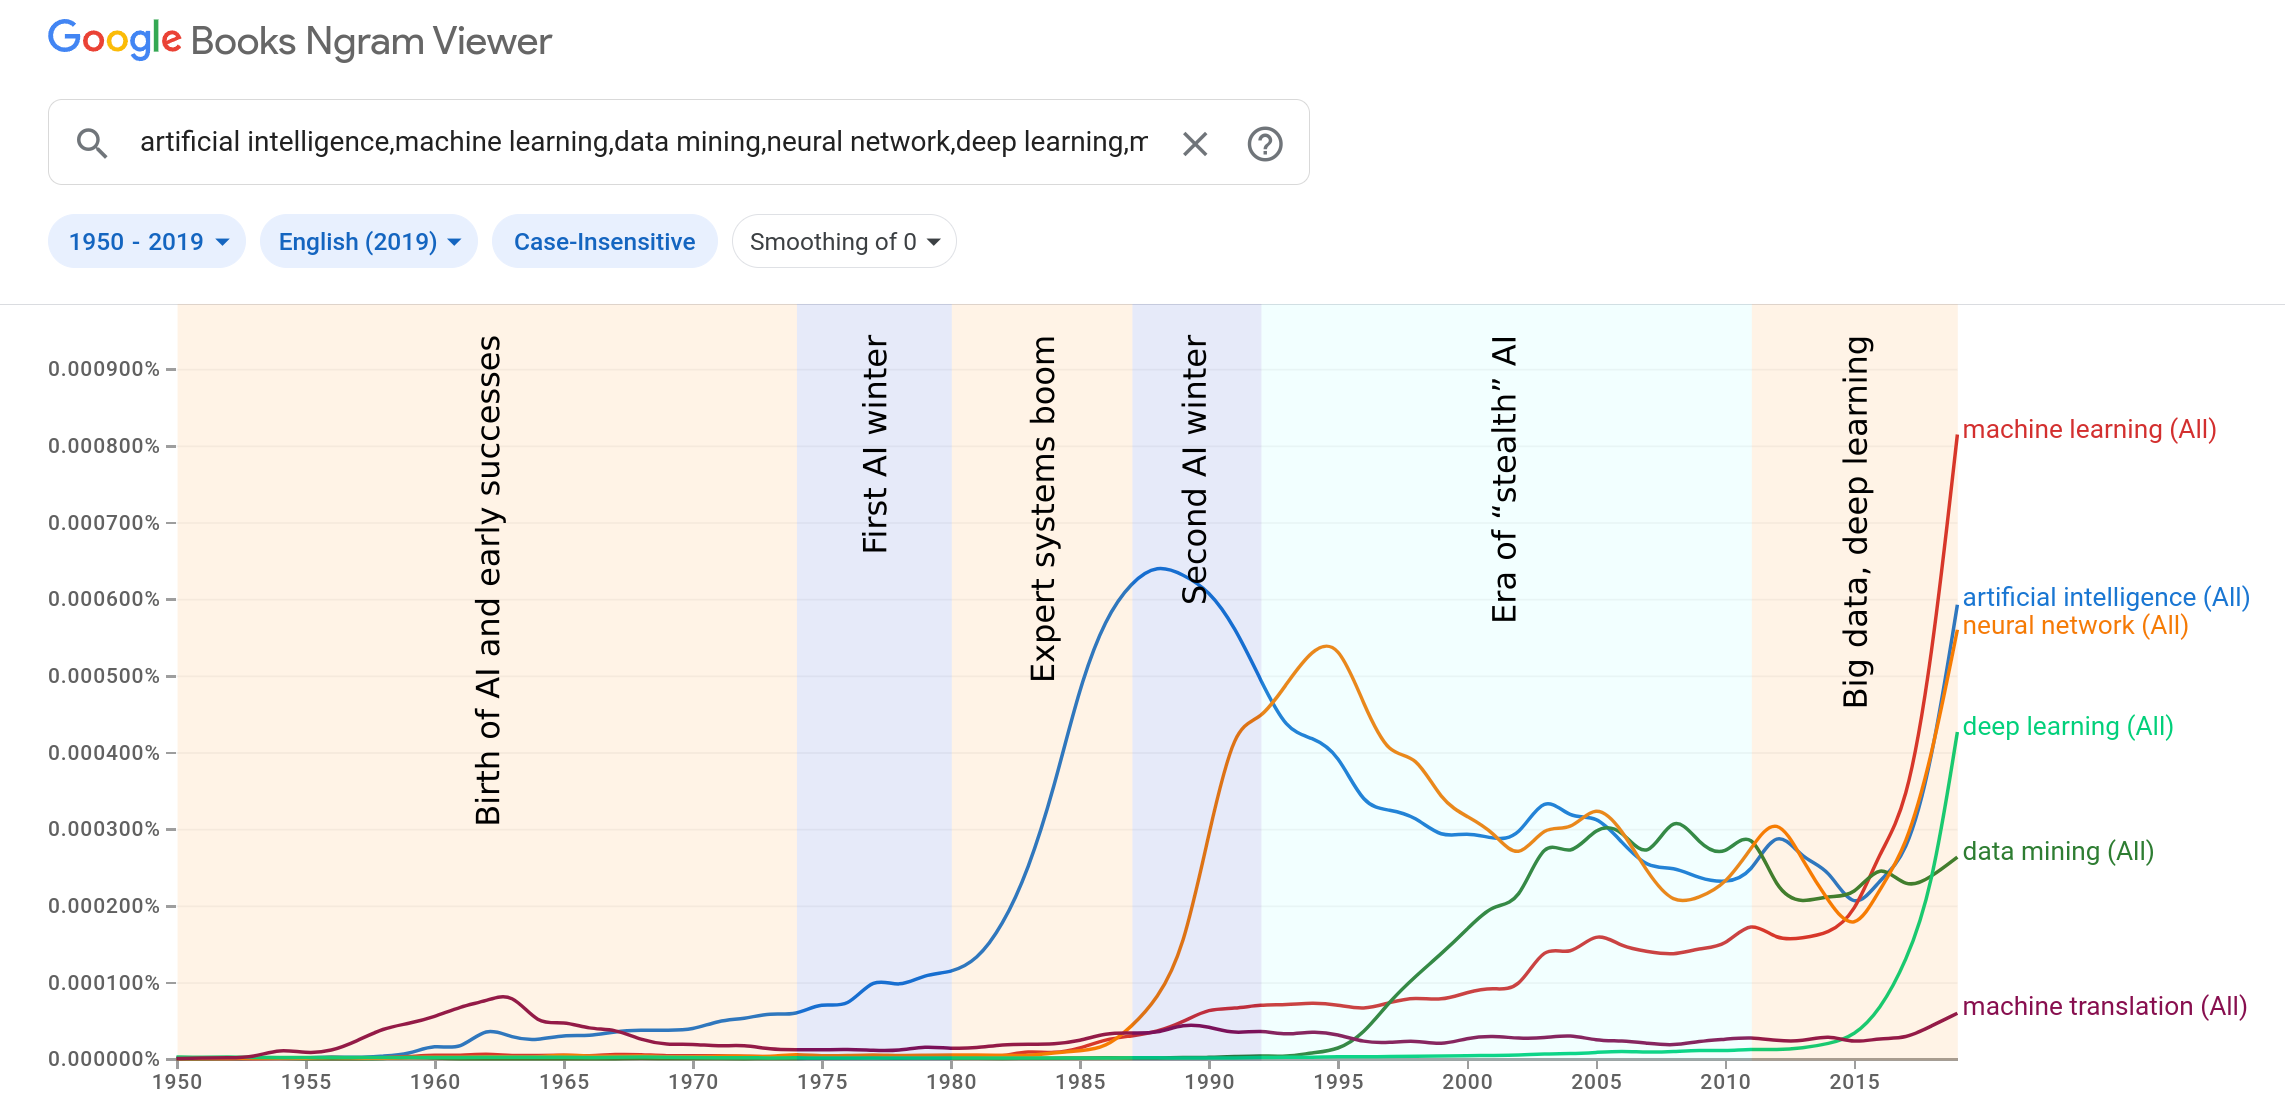
\includegraphics[width=\linewidth]{img/ups-and-downs-of-ai-overlay.png}}
\end{columns}
\end{frame}

\begin{frame}{The ups and downs of AI: in conference attendance}
\vspace{0.5 cm}
\begin{columns}
\column{1.1\linewidth}
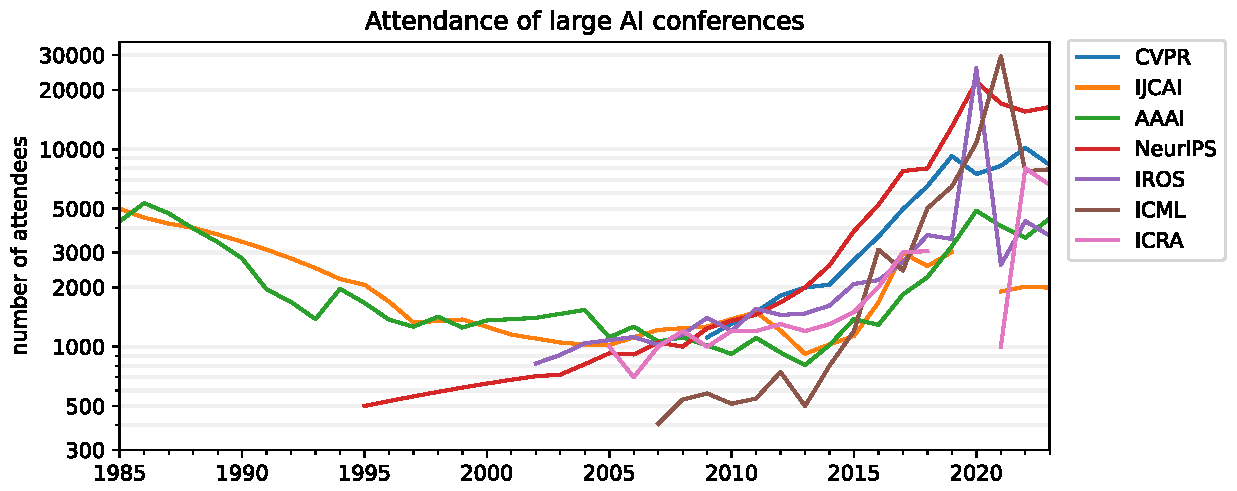
\includegraphics[width=\linewidth]{img/AI-conference-attendance.pdf}
\end{columns}
\end{frame}

\begin{frame}{The ups and downs of AI: among physicists at CHEP}
\vspace{0.25 cm}
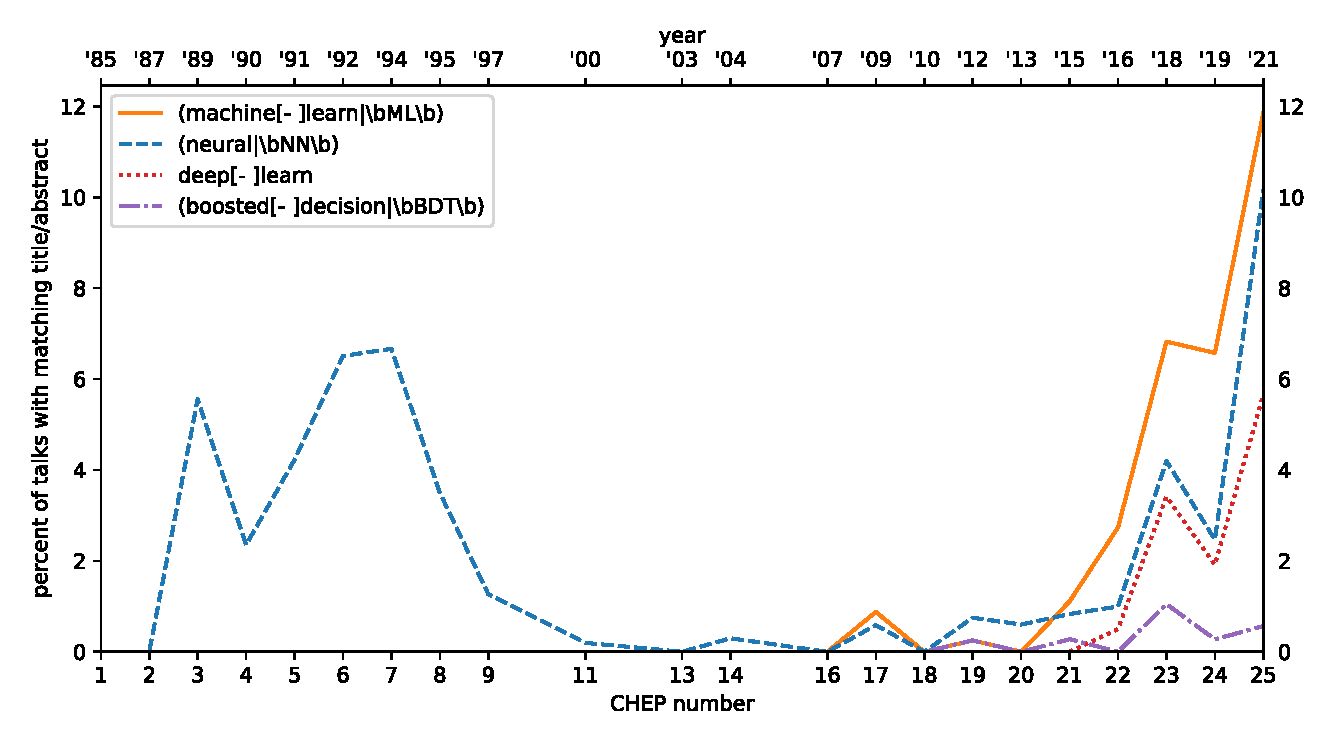
\includegraphics[width=\linewidth]{img/chep-papers-ml.pdf}
\end{frame}

\begin{frame}{Machine learning techniques that are not neural networks:}
\vspace{0.5 cm}
\large

\begin{itemize}
\item Naive Bayes classifier
\item k-nearest neighbors
\item Principal Component Analysis (PCA)
\item generalized additive models, LOWESS fitting
\item decision trees, (boosted) random forests, AdaBoost
\item k-means clustering, Gaussian processes, hierarchical clustering
\item Support Vector Machines (SVMs)
\item Hidden Markov Models (HMM)
\item {\it and many more!}
\end{itemize}

\normalsize
\vspace{0.5 cm}
\uncover<2->{(These are techniques I learned about and used when I was a data scientist, \mbox{up to 2015,\hspace{-0.2 cm}} {\it just before} the deep learning boom.)}
\end{frame}

\begin{frame}{\mbox{ }}
\begin{center}
\LARGE
In this mini-course, we'll only cover neural networks.

\large
\vspace{1 cm}
\uncover<2->{(There's enough to talk about.)}
\end{center}
\end{frame}

\begin{frame}{\mbox{ }}
\begin{center}
\LARGE
The rest of this PDF talk: \textcolor{darkblue}{what is a neural network?}

\vspace{1 cm}
Switch to Jupyter: \textcolor{darkblue}{why does a neural network work?}
\end{center}
\end{frame}

\begin{frame}{\only<1-4>{Simplest neural network is a linear fit}\only<5>{Next-simplest passes it through a non-linear function $f$}}
\vspace{0.25 cm}
\begin{onlyenv}<1>
\begin{center}
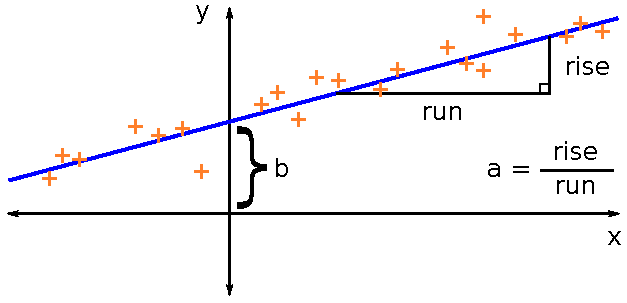
\includegraphics[width=0.4\linewidth]{img/equation-for-a-line.pdf}
\end{center}
\vspace{-1.5 cm}
\end{onlyenv}\begin{onlyenv}<2>
\begin{center}
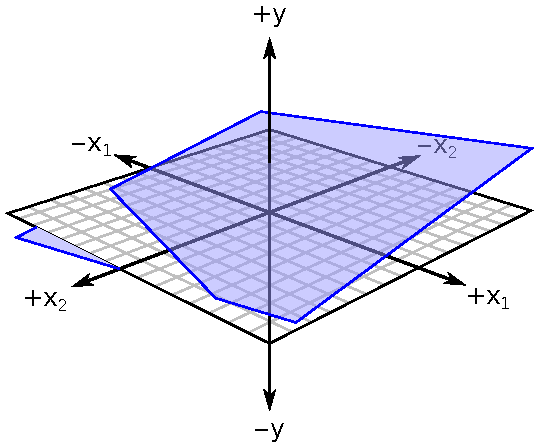
\includegraphics[width=0.4\linewidth]{img/equation-for-a-plane.pdf}
\end{center}
\vspace{-1.75 cm}
\end{onlyenv}

\begin{columns}
\column{1.1\linewidth}
\renewcommand{\arraystretch}{1.5}
\scriptsize
\[ \uncover<5->{f \left[} \mbox{\hspace{0.25 cm}} \underbrace{\uncover<2->{\left(} \begin{array}{c c c c}
\only<2->{\uncover<4->{a_{1,1}} & \uncover<4->{a_{1,2}} & \uncover<4->{\ldots} & \uncover<4->{a_{1,10}} \\}
\only<2->{\uncover<4->{a_{2,1}} & \uncover<4->{a_{2,2}} & \uncover<4->{\ldots} & \uncover<4->{a_{2,10}} \\}
\only<2->{\only<2-3>{a_1}\only<4->{a_{3,1}} & \only<2-3>{a_2}\only<4->{a_{3,2}} & \uncover<3->{\ldots} & \uncover<3->{\only<1-3>{a_{10}}}\only<4->{a_{3,10}} \\}
\only<2->{\uncover<4->{a_{4,1}} & \uncover<4->{a_{4,2}} & \uncover<4->{\ldots} & \uncover<4->{a_{4,10}} \\}
\only<2->{\uncover<4->{a_{5,1}} & \uncover<4->{a_{5,2}} & \uncover<4->{\ldots} & \uncover<4->{a_{5,10}} \\}
\end{array}\only<1>{\mbox{\hspace{0.5 cm}}a\mbox{\hspace{0.5 cm}}} \vphantom{\vbox to 1.5cm{}} \uncover<2->{\right)}}_{\text{free parameters in the fit}} \cdot \underbrace{\uncover<2->{\left(} \only<1>{x}\begin{array}{c}
\only<2->{\uncover<2->{x_1} \\}
\only<2->{\uncover<2->{x_2} \\}
\only<2->{\uncover<3->{\vdots} \\}
\only<2->{\uncover<3->{x_{10}} \\}
\end{array} \vphantom{\vbox to 1.5cm{}} \uncover<2->{\right)}}_{\text{input values}} + \underbrace{\uncover<4->{\left(} \begin{array}{c}
\uncover<4->{b_1} \\
\uncover<4->{b_2} \\
\only<1-3>{b}\only<4->{b_3} \\
\uncover<4->{b_4} \\
\uncover<4->{b_5} \\
\end{array} \vphantom{\vbox to 1.5cm{}} \uncover<4->{\right)}}_{\text{free parameters}} \mbox{\hspace{0.25 cm}} \uncover<5->{\right]} = \underbrace{\uncover<4->{\left(} \begin{array}{c}
\uncover<4->{y_1} \\
\uncover<4->{y_2} \\
\only<1-3>{y}\only<4->{y_3} \\
\uncover<4->{y_4} \\
\uncover<4->{y_5} \\
\end{array} \vphantom{\vbox to 1.5cm{}} \uncover<4->{\right)}}_{\text{output values}} = \begin{array}{c}
\uncover<5->{f[} \uncover<4->{a_{1,1}x_1 + a_{1,2}x_2 + \ldots a_{1,10}x_{10} + b_1} \uncover<5->{]} \\
\uncover<5->{f[} \uncover<4->{a_{2,1}x_1 + a_{2,2}x_2 + \ldots a_{2,10}x_{10} + b_2} \uncover<5->{]} \\
\uncover<5->{f[} \only<1>{ax + b}\only<2-3>{a_{1}x_1 + a_{2}x_2 \uncover<3->{+ \ldots a_{10}x_{10}} + b}\only<4->{a_{3,1}x_1 + a_{3,2}x_2 + \ldots a_{3,10}x_{10} + b_3} \uncover<5->{]} \\
\uncover<5->{f[} \uncover<4->{a_{4,1}x_1 + a_{4,2}x_2 + \ldots a_{4,10}x_{10} + b_4} \uncover<5->{]} \\
\uncover<5->{f[} \uncover<4->{a_{5,1}x_1 + a_{5,2}x_2 + \ldots a_{5,10}x_{10} + b_5} \uncover<5->{]} \\
\end{array} \]
\end{columns}
\end{frame}

\begin{frame}{The non-linear function $f$ is called an ``activation function''}
\small
\vspace{0.5cm}
\begin{columns}
\column{0.2\linewidth}
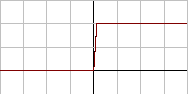
\includegraphics[width=\linewidth]{img/Activation_binary_step.pdf}

\column{0.25\linewidth}
binary step

\vspace{-\baselineskip}
\[ f(x) = \left\{ \begin{array}{c l}
0 & \text{if } x < 0 \\
1 & \text{if } x \ge 0 \\
\end{array} \right. \]

\column{0.2\linewidth}
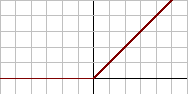
\includegraphics[width=\linewidth]{img/Activation_rectified_linear.pdf}

\column{0.3\linewidth}
rectified linear unit (ReLU)

\vspace{-\baselineskip}
\[ f(x) = \left\{ \begin{array}{c l}
0 & \text{if } x < 0 \\
x & \text{if } x \ge 0 \\
\end{array} \right. \]
\end{columns}

\vspace{0.5cm}
\begin{columns}
\column{0.2\linewidth}
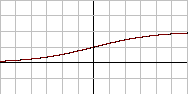
\includegraphics[width=\linewidth]{img/Activation_logistic.pdf}

\column{0.25\linewidth}
logistic (soft step)

\vspace{-\baselineskip}
\[ f(x) = \frac{1}{1 + e^{-x}} \]

\column{0.2\linewidth}
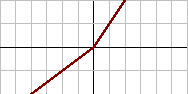
\includegraphics[width=\linewidth]{img/Activation_prelu.pdf}


\column{0.3\linewidth}
``leaky'' ReLU

\vspace{-\baselineskip}
\[ f(x) = \left\{ \begin{array}{c l}
\alpha x & \text{if } x < 0 \\
x & \text{if } x \ge 0 \\
\end{array} \right. \]
\end{columns}

\vspace{0.5cm}
\begin{columns}
\column{0.2\linewidth}
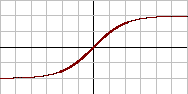
\includegraphics[width=\linewidth]{img/Activation_tanh.pdf}

\column{0.25\linewidth}
hyperbolic tangent

\vspace{-\baselineskip}
\[ f(x) = \frac{e^x - e^{-x}}{e^x + e^{-x}} \]

\column{0.2\linewidth}
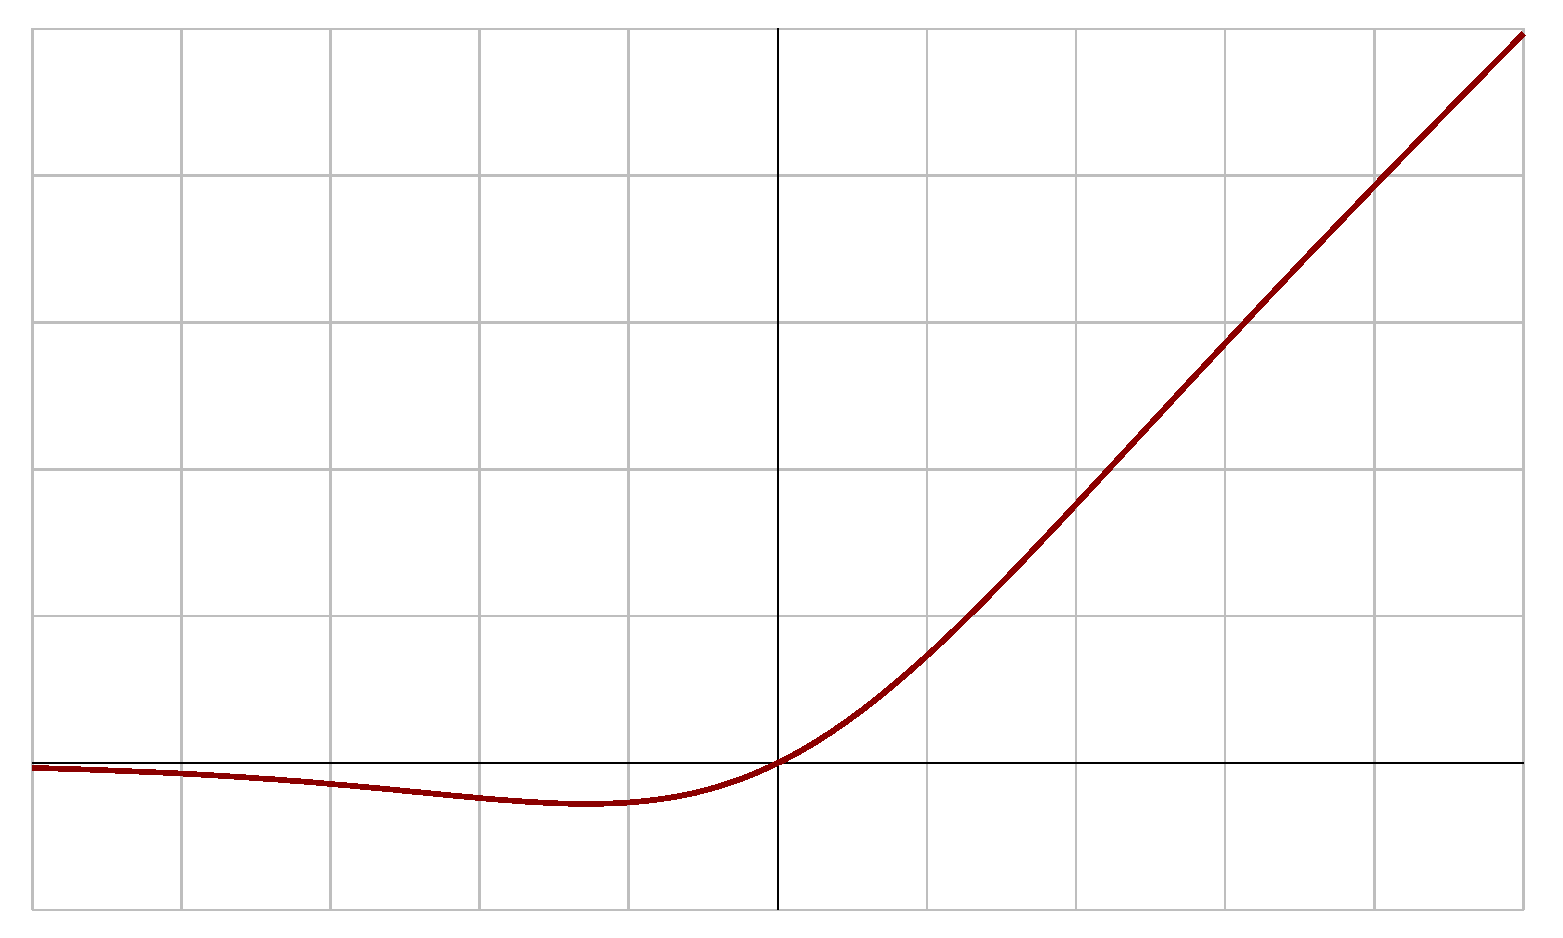
\includegraphics[width=\linewidth]{img/Activation_swish.pdf}

\column{0.3\linewidth}
sigmoid linear unit (``swish'')

\[ f(x) = \frac{x}{1 + e^{-x}} \]
\end{columns}

\large

\vspace{0.75 cm}
There are many choices, but ReLU is the simplest and most common.
\end{frame}

\begin{frame}{Neural networks take inspiration from neurons in the brain}
\begin{center}
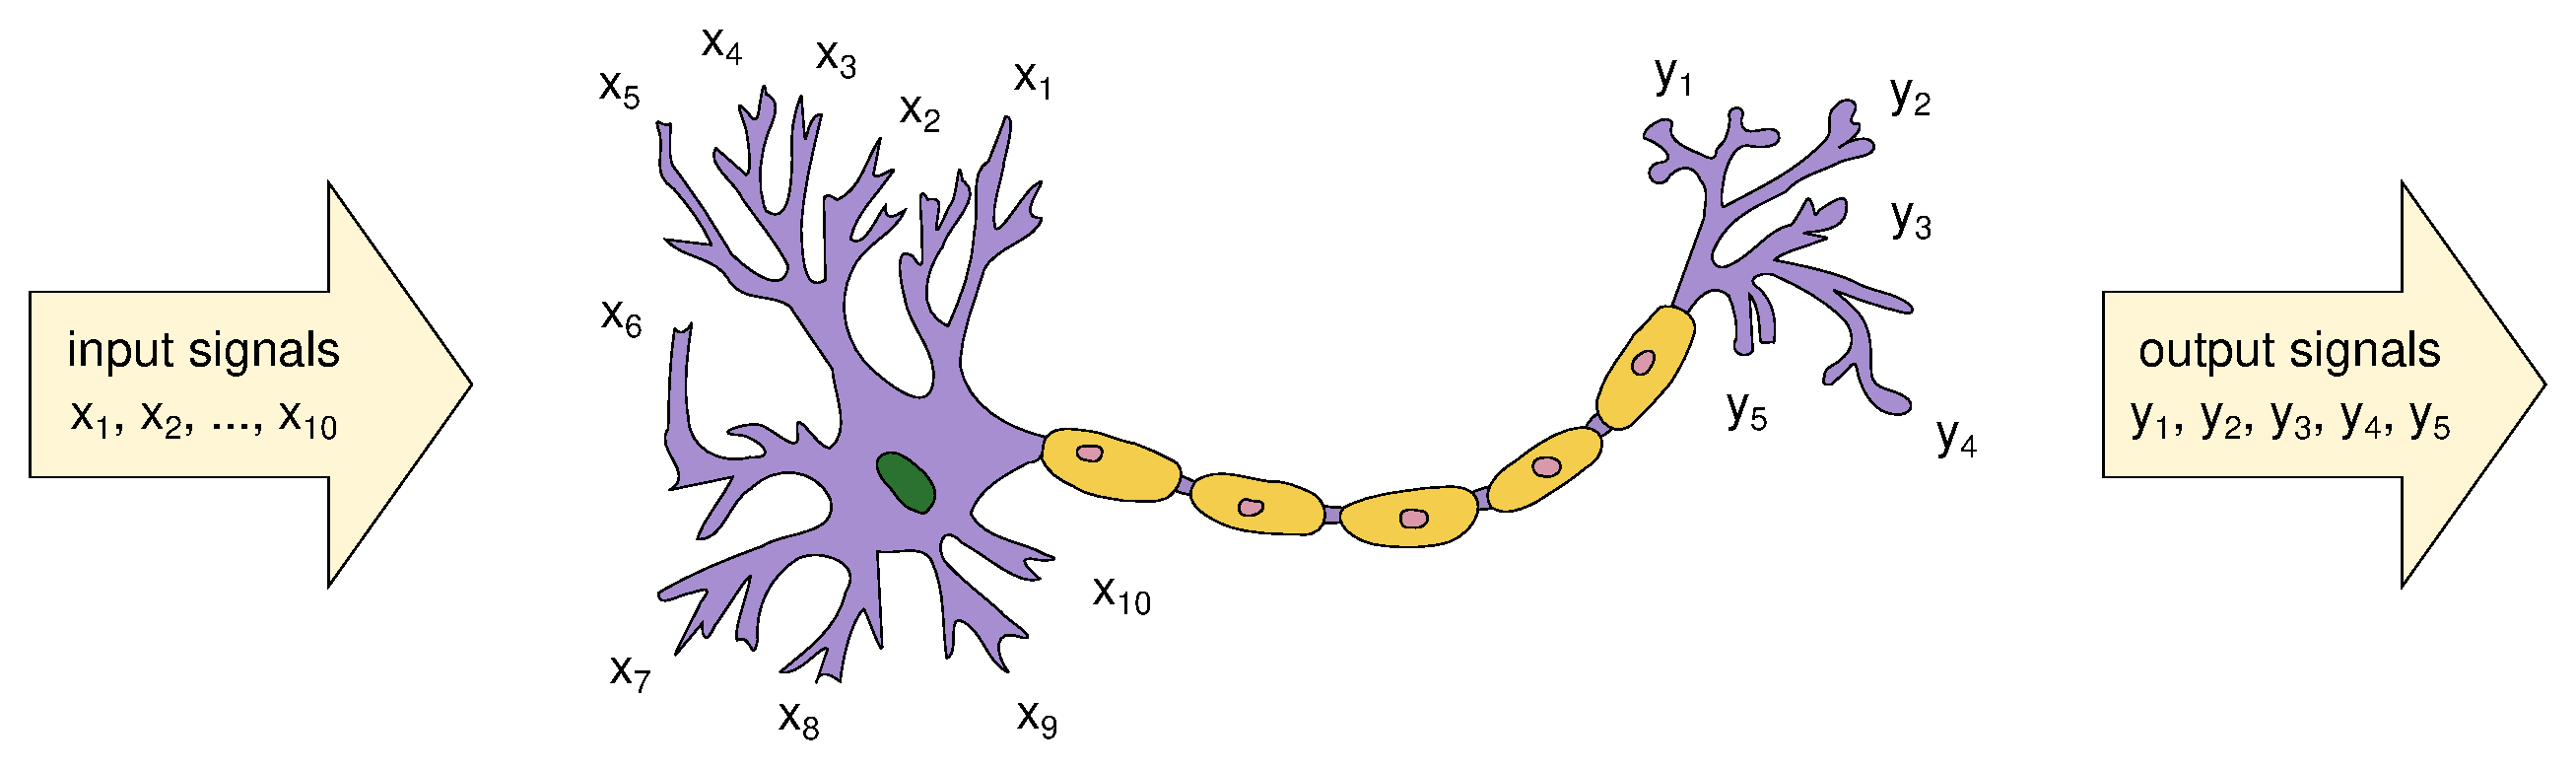
\includegraphics[width=0.9\linewidth]{img/real-neuron.pdf}
\end{center}

\vspace{-1cm}
\begin{columns}
\column{1.1\linewidth}
\renewcommand{\arraystretch}{1.5}
\scriptsize
\[ f \left[ \mbox{\hspace{0.25 cm}} \underbrace{\left( \begin{array}{c c c c}
a_{1,1} & a_{1,2} & \ldots & a_{1,10} \\
a_{2,1} & a_{2,2} & \ldots & a_{2,10} \\
a_{3,1} & a_{3,2} & \ldots & a_{3,10} \\
a_{4,1} & a_{4,2} & \ldots & a_{4,10} \\
a_{5,1} & a_{5,2} & \ldots & a_{5,10} \\
\end{array} \vphantom{\vbox to 1.5cm{}} \right)}_{\text{free parameters in the fit}} \cdot \underbrace{\left( \begin{array}{c}
x_1 \\
x_2 \\
\vdots \\
x_{10} \\
\end{array} \vphantom{\vbox to 1.5cm{}} \right)}_{\text{input values}} + \underbrace{\left( \begin{array}{c}
b_1 \\
b_2 \\
b_3 \\
b_4 \\
b_5 \\
\end{array} \vphantom{\vbox to 1.5cm{}} \right)}_{\text{free parameters}} \mbox{\hspace{0.25 cm}} \right] = \underbrace{\left( \begin{array}{c}
y_1 \\
y_2 \\
y_3 \\
y_4 \\
y_5 \\
\end{array} \vphantom{\vbox to 1.5cm{}} \right)}_{\text{output values}} = \begin{array}{c}
f[ a_{1,1}x_1 + a_{1,2}x_2 + \ldots a_{1,10}x_{10} + b_1 ] \\
f[ a_{2,1}x_1 + a_{2,2}x_2 + \ldots a_{2,10}x_{10} + b_2 ] \\
f[ a_{3,1}x_1 + a_{3,2}x_2 + \ldots a_{3,10}x_{10} + b_3 ] \\
f[ a_{4,1}x_1 + a_{4,2}x_2 + \ldots a_{4,10}x_{10} + b_4 ] \\
f[ a_{5,1}x_1 + a_{5,2}x_2 + \ldots a_{5,10}x_{10} + b_5 ] \\
\end{array} \]
\end{columns}
\end{frame}

\begin{frame}{Neural networks take inspiration from neurons in the brain}
\vspace{0.15 cm}
\begin{columns}
\column{1.2\linewidth}
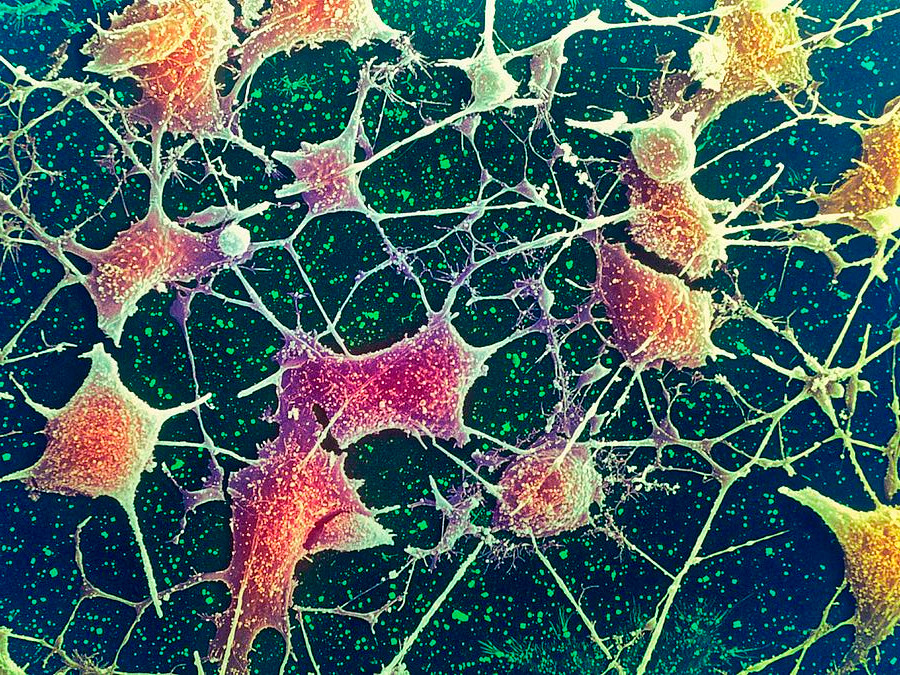
\includegraphics[width=\linewidth]{img/nerve-cells-sem-steve-gschmeissner.jpg}
\end{columns}
\end{frame}

\begin{frame}{Neural networks take inspiration from neurons in the brain}
\vspace{0.16 cm}
\begin{columns}
\column{1.1\linewidth}
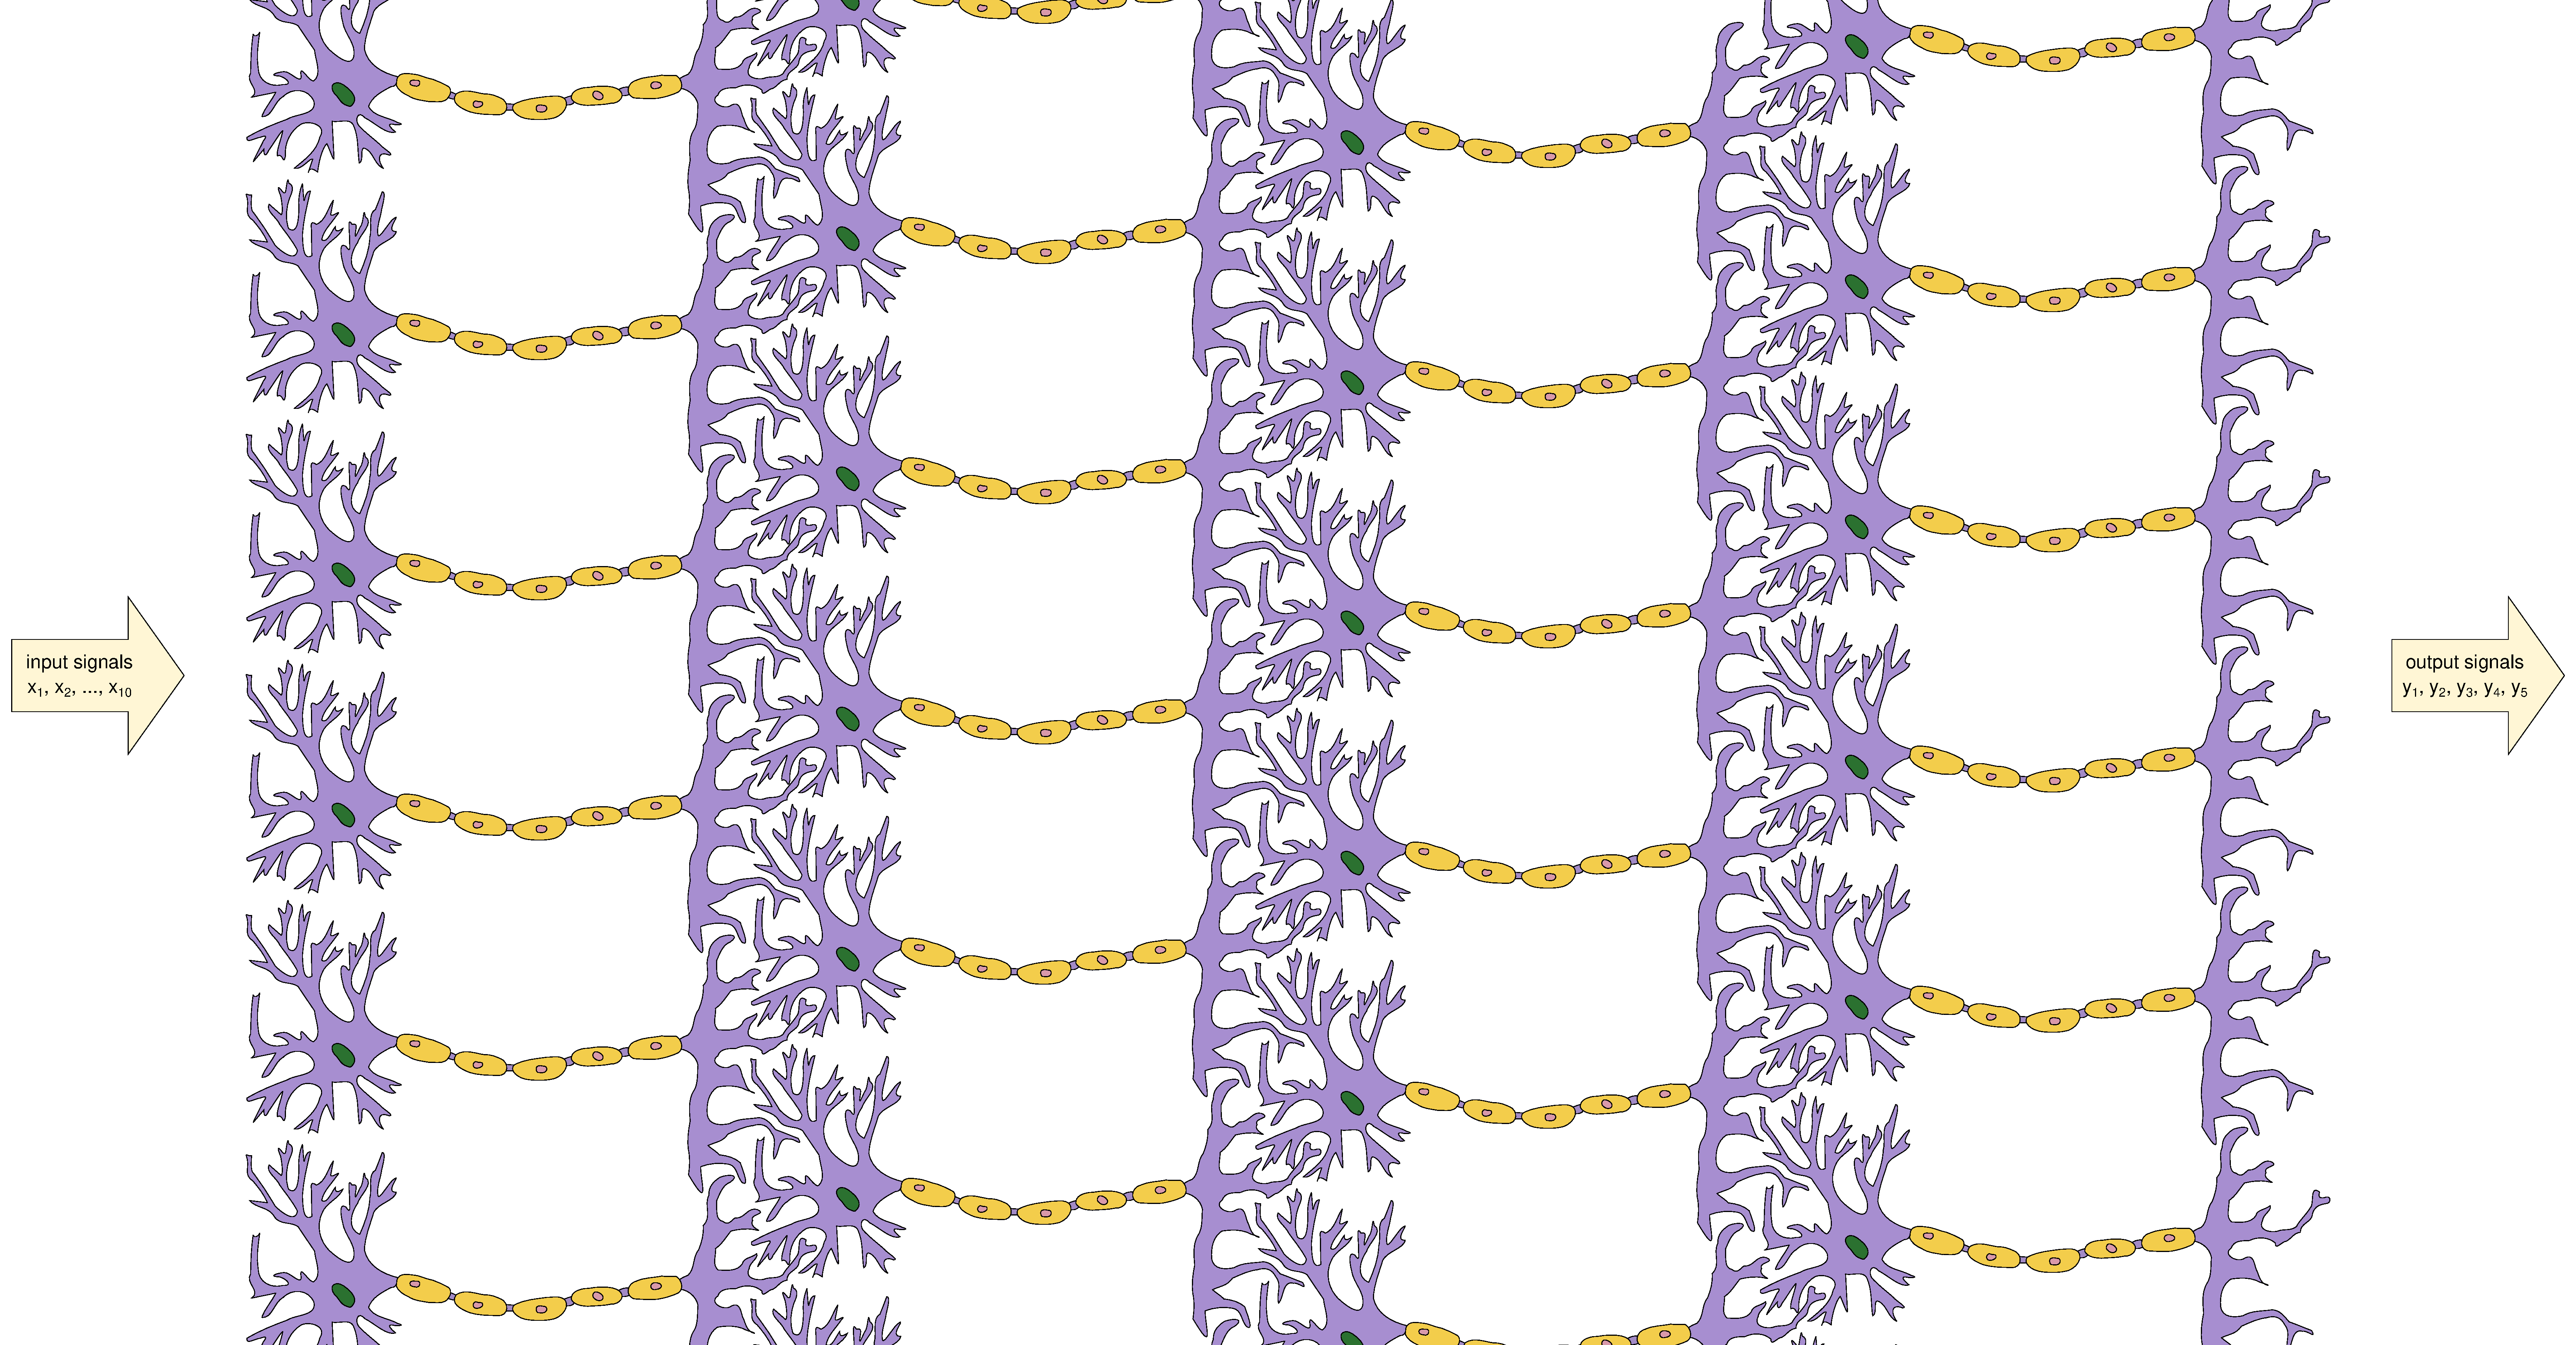
\includegraphics[width=\linewidth]{img/real-neuron-layers.pdf}
\end{columns}
\end{frame}

\begin{frame}{Neural networks take inspiration from neurons in the brain}
To do the same thing with our model, take the output of one ``activation + linear transform'' and use it as the input to the next:

\vspace{1 cm}
\begin{columns}
\column{1.15\linewidth}
\[ \only<1>{f \left( a^{\text{layer 1}}_{i\mbox{,\,}j} \cdot x_j + b^{\text{layer 1}}_i \right)}\only<2>{f \left( a^{\text{layer 2}}_{i\mbox{,\,}j} \cdot \fbox{$\displaystyle f \left( a^{\text{layer 1}}_{i\mbox{,\,}j} \cdot x_j + b^{\text{layer 1}}_i \right)$} + b^{\text{layer 2}}_i \right)}\only<3>{f \left( a^{\text{layer 3}}_{i\mbox{,\,}j} \cdot \fbox{$\displaystyle f \left( a^{\text{layer 2}}_{i\mbox{,\,}j} \cdot \fbox{$\displaystyle f \left( a^{\text{layer 1}}_{i\mbox{,\,}j} \cdot x_j + b^{\text{layer 1}}_i \right)$} + b^{\text{layer 2}}_i \right) $} + b^{\text{layer 3}}_i \right)}\only<4->{\mbox{\hspace{-1 cm}}f \left( a^{\text{layer 4}}_{i\mbox{,\,}j} \cdot \fbox{$\displaystyle f \left( a^{\text{layer 3}}_{i\mbox{,\,}j} \cdot \fbox{$\displaystyle f \left( a^{\text{layer 2}}_{i\mbox{,\,}j} \cdot \fbox{$\displaystyle f \left( a^{\text{layer 1}}_{i\mbox{,\,}j} \cdot x_j + b^{\text{layer 1}}_i \right)$} + b^{\text{layer 2}}_i \right) $} + b^{\text{layer 3}}_i \right) $} + b^{\text{layer 4}}_i \right)\mbox{\hspace{-1 cm}}} \]
\end{columns}

\vspace{1 cm}
\uncover<5>{Without the activation functions, we'd lose the structure: linear transformations of linear transformations collapse down to a single linear transformation.}

\end{frame}

\begin{frame}{It's usually drawn like this}
\vspace{0.25 cm}
\only<1>{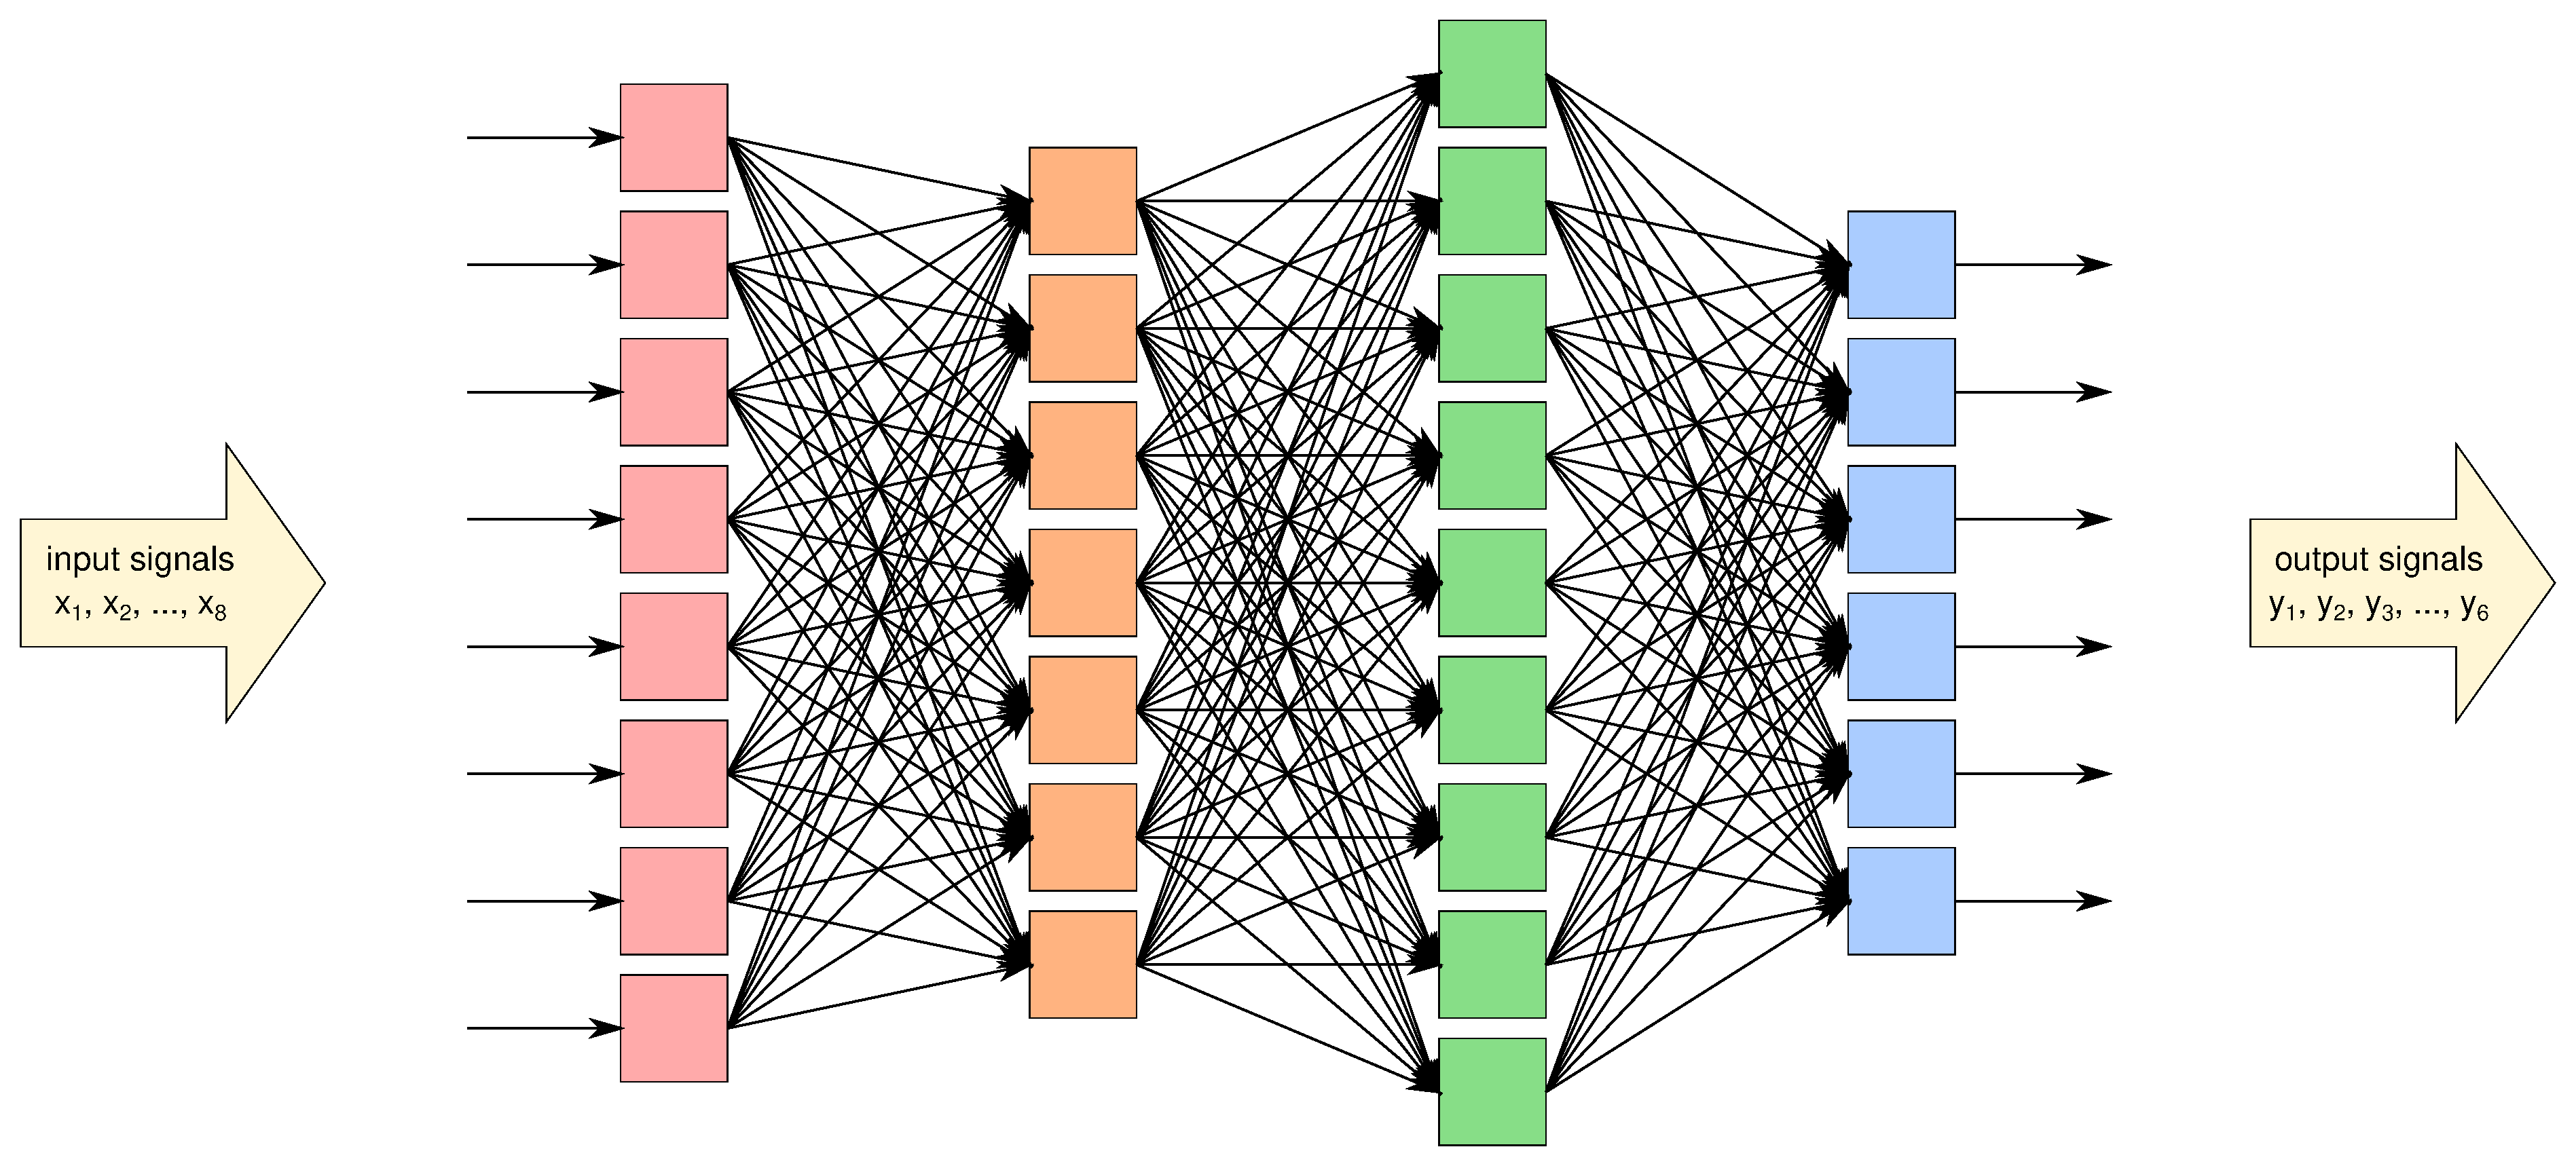
\includegraphics[width=\linewidth]{img/artificial-neural-network-layers.pdf}}\only<2>{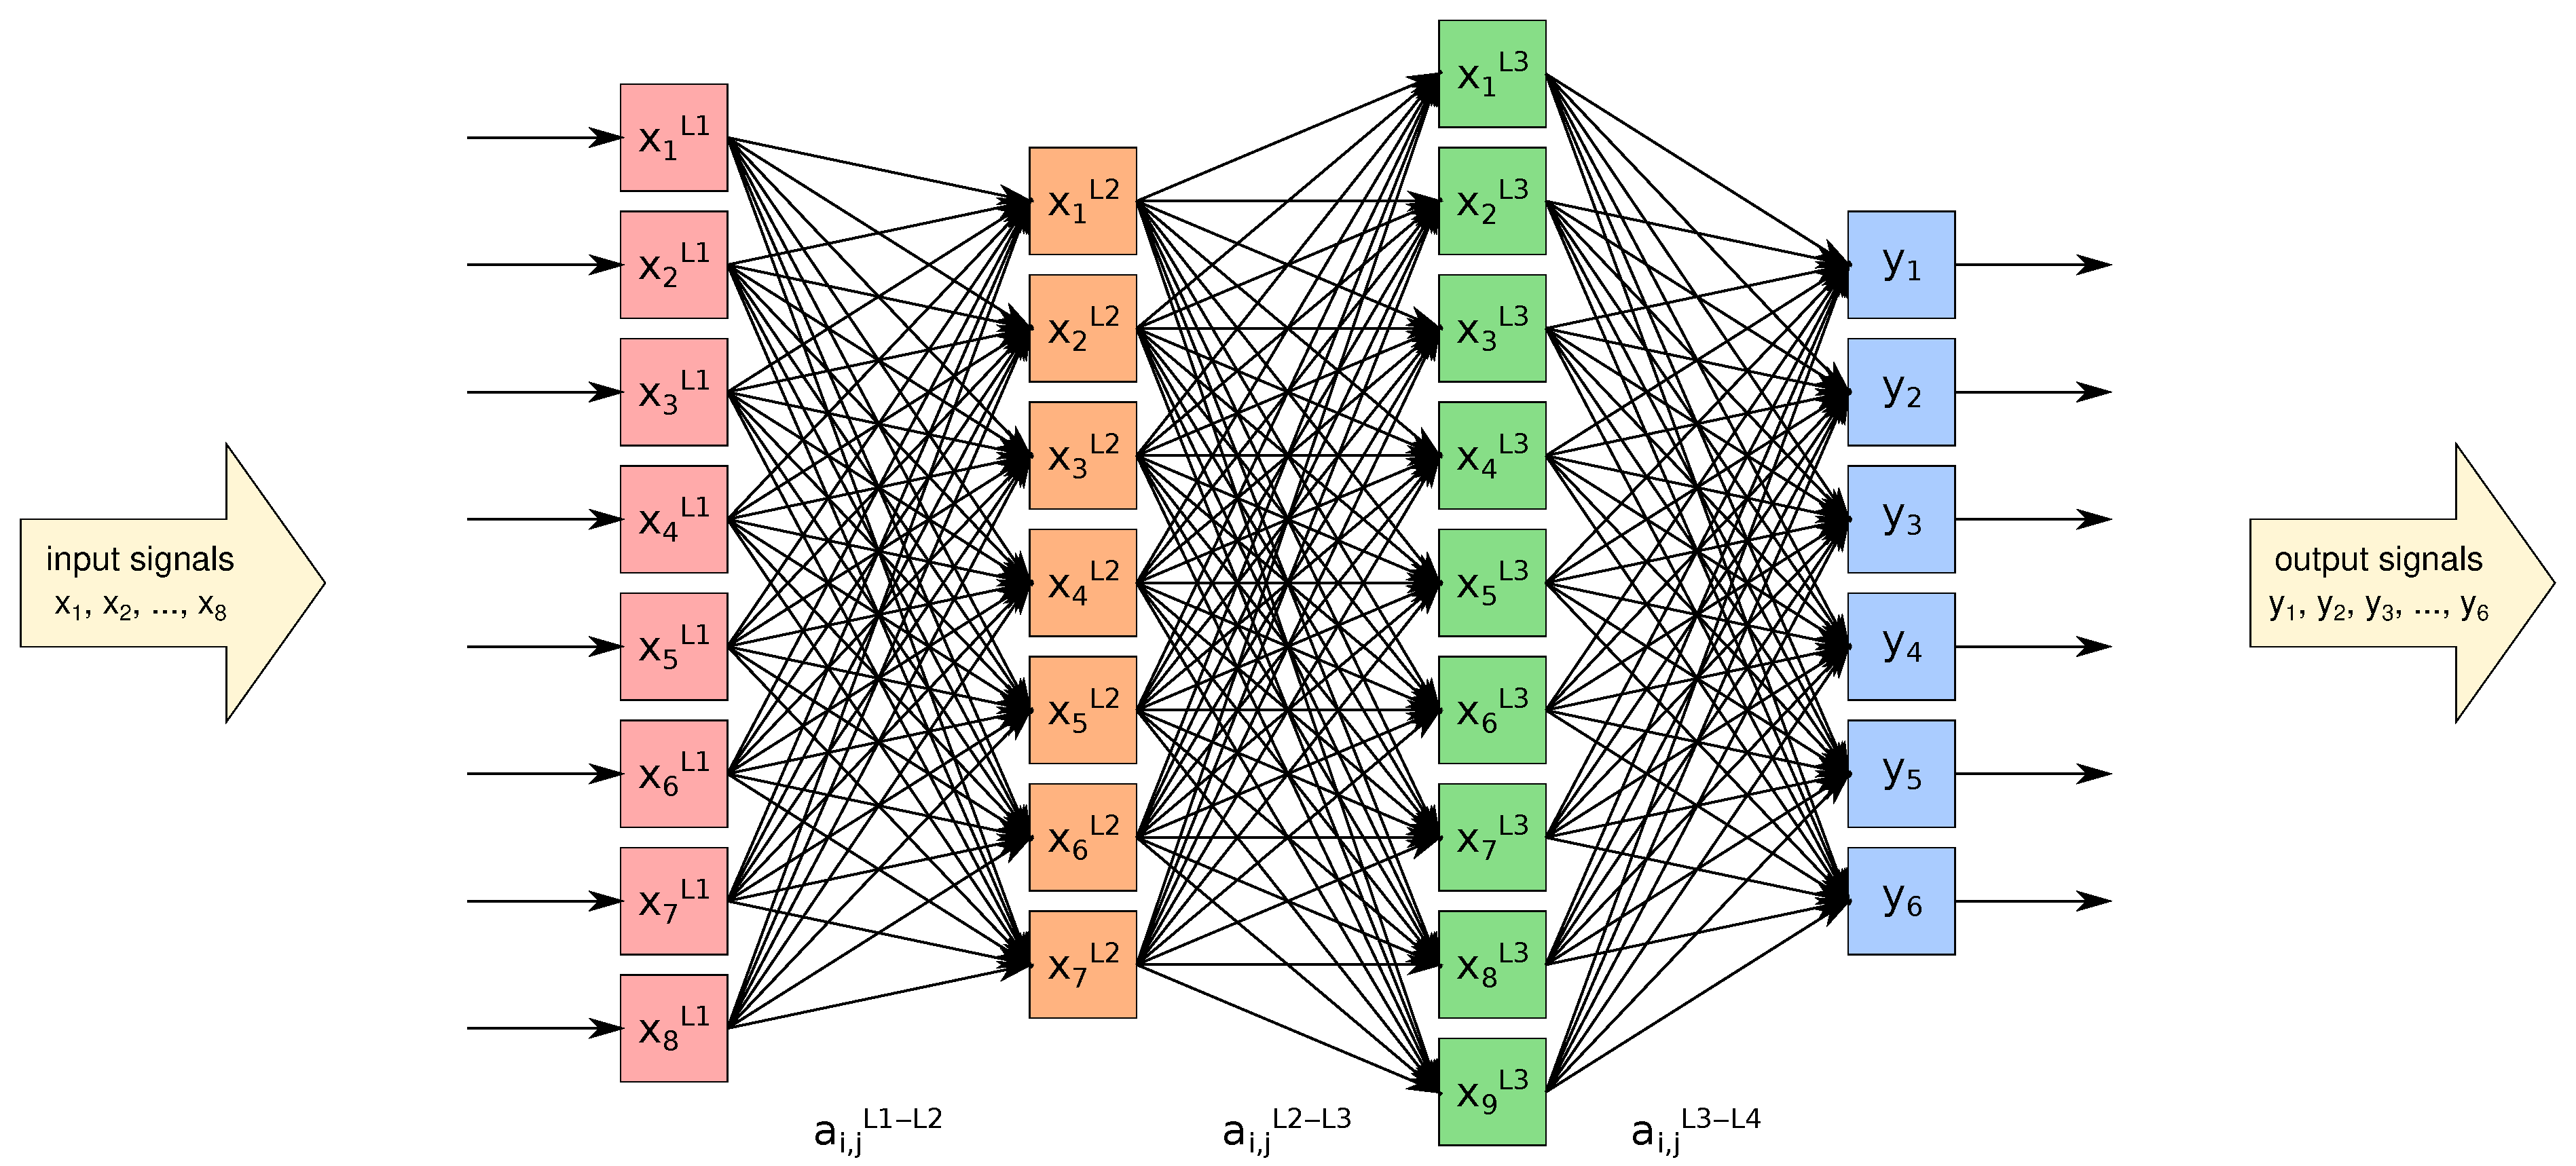
\includegraphics[width=\linewidth]{img/artificial-neural-network-layers-2.pdf}}

\vspace{0.25 cm}
The lines indicate that every output from one layer is included in the linear transformation of the next layer. (``There's an $a_{i\mbox{,\,}j}$ for every $x_j$ and $y_i$.'')
\end{frame}

\begin{frame}{\mbox{ }}
\begin{center}
\LARGE
But\ldots why does that work?

\vspace{1 cm}
What's so special about this linear-nonlinear sandwich?

\vspace{1 cm}
\large
\uncover<2->{\textcolor{darkblue}{(Time to switch to Jupyter.)}}
\end{center}
\end{frame}

\end{document}
